\section{Pr\'elude: Primes in integral extensions}
    \subsection{Behaviours of prime ideals in integral extensions}
        \subsubsection{Finite and integral extensions}
            \begin{definition}[Integral extensions] \label{def: integral_extensions} \index{Integral! extensions} \index{Integral! elements}
                \noindent
                \begin{enumerate}
                    \item \textbf{(Integral elements):} Let $A$ be a subring of a commutative ring $B$ (i.e. let their exist monic ring homomorphisms from $A$ to $B$). An element $b \in B$ will be called \textbf{integral} over $A$ if and only if $A[b]$ is a finitely generated commutative $A$-algebra; otherwise, it is called \textbf{transcendental}. When $A$ is a field, what one recovers are the notions of algebraic and transcendental elements (for instance, $\sqrt{2}$ is integral over $\Z$, as it is algebraic over $\Q$, whereas a formal variable $x$ is neither). 
                    \item \textbf{(Integral extensions):} A homomorphism between commutative rings $A \to B$ will be called an integral extension if all elements of $B$ are integral over $B$. Alternatively (and perhaps less confusingly), one may view an integral extension of a commutative ring $A$ as a tensor product $\bigotimes_{i \in I} A[b_i]$ wherein $\{b_i\}_{i \in I}$ is a (possibly infinite) set of elements that are integral over $A$; note that one has the following canonical isomorphism of commutative $A$-algebras:
                        $$\bigotimes_{i \in I} A[b_i] \cong A\left[\{b_i\}_{i \in I}\right]$$
                    thanks to the fact that left-adjoints (the polynomial ring free construction) commutes with colimits (tensor products of commutative algebras). Additionally, integral extensions are trivially injective ring homomorphisms.
                    \item \textbf{(Integral closures):} Let $\varphi: A \to B$ be a homomorphism of commutative rings. Then, the integral closure of $A$ inside $B$ (denoted by $\overline{A}$, $\overline{A_B}$, or $\overline{A_{\varphi}}$) is the subset of $B$ consisting of \textit{all} elements that are integral over $A$. It is not hard to show that integral closures are actually subrings of the codomains, and with this in mind, one can see that integral closures may be viewed as maximal integral extensions inside given commutative rings; this description can be succinctly summed up by the following expression:
                        $$\overline{A_{\varphi}} \cong \bigotimes_{\underset{\text{$b$ integral over $\im \varphi$}}{b \in B}} A[b]$$
                \end{enumerate}
            \end{definition}
            \begin{example}[The ring of integers of a number field] \label{example: ring_of_integers}
                \noindent
                \begin{enumerate}
                    \item \textbf{(The global case):} Before we try to give a description of rings of integers inside global fields, let us fix a definition. To us, a global field is either a finite (hence \textit{a priori} algebraic) extension of $\Q$ or of $\F_p(t)$, the field of Laurent series with coefficients coming from the finite field of prime order $p$. With this definition in mind, let us then define the ring of integers of a global field $F$ as the maximal commutative ring (in terms of cardinality) that is integrally closed inside $F$. For example, $\Z$ is the ring of integers of $\Q$, but $\Z$ is not of $\R$ (not that $\R$ is a global field, nor can we even define the ring of integers of $\R$ anyway). This definition, while conceptually intuitive, is not very practical. That is because it is not entirely clear how one might trickle from a given global field down onto its largest subring that is integrally closed. Thus, one can define the ring of integers $\scrO_F$ of a global field $F$ alternatively as the set of all elements of $F$ that are integral over $\Z$ (in the event that $\chara F = 0$) or over $\F_p[t]$ (if $\chara F = p$, for some prime $p$). Per this definition, rings of integers are automatically closed inside their corresponding global fields. Furthermore, all global fields are equal to the field of fractions of their rings of integers.
                    \item \textbf{(The local case):} As above, let us first try to agree upon a notion of local fields: an \textit{archimedean} local field is a finite extension of $\R$ (so actually, just $\R$ and $\bbC$), and a \textit{non-archimedean} local field is either a finite extension of $\Q_p$ (i.e. a $p$-adic number field) - which we note to be of mixed characteristic $(0,p)$ - or a finite extension of $\F_p(\!(t))\!$ - which we note to be of equicharacteristic $(p, p)$ - i.e. the field of formal Laurent series over the finite field of order $p$. One can do some work to see that given a local field $K$, one can define a suitable sort of \say{absolute value} $|-|$ on it, and with respect to such an absolute value, one obtains either an archimedean metric topology or a non-archimedean ultrametric topology (hence the names). Then, consider the \textit{closed} unit ball inside $K$, i.e. the set:
                        $$\scrO_K := \{x \in K \mid |x| \leq 1\}$$
                    (for instance, $\Z_p$ and $\F_p[\![t]\!]$ are the closed unit balls inside $\Q_p$ and $\F_p(\!(t)\!)$ respectively, and $[-1, 1]$ is the the unit ball inside $\R$). In the non-archimedean case, this turns out to be a subring of $K$, which we dub the ring of integers of $K$. Interestingly, the ring of integers of a non-archimedean local field is integrally closed and one can show this by first showing that the \textit{open} unit ball inside $K$, i.e. the set:
                        $$\m_K := \{x \in K \mid |x| < 1\}$$
                    is the (necessarily unique) maximal ideal of $\scrO_K$; then, 
                    \\
                    Of course, one could also define the ring of integers of a non-archimedean local field $K$ as the set of all elements in $K$ that are integral over either $\Z_p$ or $\F_p[\![t]\!]$ (corresponding to $\chara K = 0$ and $\chara K = p$ respectively) and then show that such elements would have their absolute values bounded above by $1$. 
                \end{enumerate}
                
                One interesting object that can be built out of global fields, local fields, along with rings of integers thereof are rings of a\`eles of global fields: the ring of ad\`eles of a global field $F$ is defined to be the following so-called \textbf{restricted product}:
                    $$\A_F := \hat{\prod_{v \in \Spec \scrO_F}} F_v := \underset{V \in \calP^{\fin}_{\Spec \scrO_F}}{\colim} \left(\prod_{v \in V} F_v \x \prod_{v \in \Spec \scrO_F \setminus V} \scrO_{F, v}\right)$$
                wherein $\calP^{\fin}_{\Spec \scrO_F}$ is the poset of \textit{finite} subsets of $\Spec \scrO_F$, and for each place $v \in \Spec \scrO_F$, one writes $F_v$ for the $v$-adic completion of $F$ and $\scrO_{F, v}$ for the ring of integers of $F_v$. For instance, the ring of ad\`eles of $\Q$ is:
                    $$\A_{\Q} := \hat{\prod_{p \in \Spec \Z}} \Q_p := \underset{V \in \calP^{\fin}_{\Spec \Z}}{\colim} \left(\prod_{p \in V} \Q_p \x \prod_{q \in \Spec \scrO_F \setminus V} \Z_q\right)$$
            \end{example}
            \begin{example}[More instances of integrality]
                \noindent
                \begin{enumerate}
                    \item \textbf{(Dedekind domains):} Any Dedekind domain is integrally closed in its field of fractions. However, this is not the case for general integral domains, i.e. there are integral domains which are not 
                    \item \textbf{(Algebraic closures):} Because algebraic extensions are special cases of integral extensions, algebraic closures are nothing but instances of integral closures.
                    \item \textbf{(The ring of integers of a number field):} We have seen in example \ref{example: ring_of_integers} that given any number field $E$, the corresponding ring of integers $\scrO_E$ is its own integral closure in $E$. Let us now examine a few concrete instances of this phenomenon:
                        \begin{enumerate}
                            \item \textbf{(The Gaussian integers):} The ring of integers 
                            \item \textbf{(Quadratic extensions):}
                            \item \textbf{(Cyclotomic extensions):}
                            \item \textbf{(Algebraic integers):} The integral closure of $\Z$ inside the field $\overline{\Q}$ of algebraic numbers is the ring of algebraic integers (or in order to avoid tautological statements, the ring of integers of $\overline{\Q}$); one may draw the following diagram to understand the relationship between this example and that of $\Z$ inside $\Q$:
                                $$
                                    \begin{tikzcd}
                                    	\overline{\Q} & {\scrO_{\overline{\Q}}} \\
                                    	\Q & \Z
                                    	\arrow[no head, from=2-1, to=1-1]
                                    	\arrow[no head, from=2-2, to=1-2]
                                    	\arrow[no head, from=1-1, to=1-2]
                                    	\arrow[no head, from=2-1, to=2-2]
                                    \end{tikzcd}
                                $$
                        \end{enumerate}
                \end{enumerate}
            \end{example}
            \begin{remark}[Finiteness and integrality] \label{remark: finite_implies_integral}
                As it is the case with fields, finite extensions of commutative rings are integral, but the converse is not necessarily true. For instance, the extension $\Z[\{\sqrt{p}\}_{(p) \in \Spec \Z}]$ is certainly integral inside $\Q$, but definitely not finite. 
            \end{remark}
            \begin{convention}
                From now on, integral extensions will be denoted like how field extensions are, i.e. as \say{quotients}.
            \end{convention}
            
            \begin{proposition}[Equivalent definitions of integrality]
                Let $A$ be a subring of a commutative ring $B$ and let $b$ be an element of $B$. Then:
                    \begin{enumerate}
                        \item $b$ is integral over $A$ if and only if it is a root of a polynomial in $A[x]$. 
                        \item There exists a faithful $A[b]$-module that is finitely generated over $A$. 
                    \end{enumerate}
            \end{proposition}
                \begin{proof}
                                
                \end{proof}
            
            \begin{proposition}
                Compositions of integral extensions are themselves integral extensions. 
            \end{proposition}
                \begin{proof}
                                
                \end{proof}
            
            \begin{proposition}[Integrality and localisations]
                Let $A$ be a subring of a commutative ring $B$, let $\overline{A}$ denote the integral closure of $A$ inside $B$, and let $S$ be a multiplicative subset of $A$. Then, the integral closure of $S^{-1}A$ inside $S^{-1}$ is just $S^{-1}\overline{A}$. 
            \end{proposition}
                \begin{proof}
                                
                \end{proof}
            
        \subsubsection{Lying Over, Going Up, and Going Down}
            \begin{definition}[Primes lying over one another]
                Let $\pi: \Spec B \to \Spec A$ be a morphism of affine schemes. Then, a prime $\q \in |\Spec B|$ is said to lie over a prime $\p \in |\Spec A|$ if:
                    $$\q \in |\pi|^{-1}(\p)$$
            \end{definition}
        
            \begin{definition}[Going Up and Going Down]
                Let $\varphi: A \to B$ be a homomorphism between commutative rings.
                    \begin{enumerate}
                        \item \textbf{(Going Up):} $\varphi$ is said to satisfy \textbf{Going Up} if for every pair of prime ideals $\p \subset \p'$ of $A$ and for every prime $\q$ lying over $\p$, there exists a prime ideal $\q'$ above $\p'$ such that $\q' \supset \q$.  
                        \item \textbf{(Going Down):} $\varphi$ is said to satisfy \textbf{Going Down} if for every pair of prime ideals $\p \subset \p'$ of $A$ and for every prime $\q'$ lying over $\p'$, there exists a prime ideal $\q$ above $\p$ such that $\q \subset \q'$. 
                    \end{enumerate}
            \end{definition}
            
            \begin{proposition}[Going Up and Going Down criteria] \label{prop: going_up_and_down_criteria}
                \noindent
                \begin{enumerate}
                    \item Integral (and hence finite; see remark \ref{remark: finite_implies_integral} for details) extensions satisfy Going Up.
                    \item Quotient maps satisfy Going Up.
                    \item Flat ring maps (and hence localisations; see \cite{stacks}, \href{https://stacks.math.columbia.edu/tag/00HT}{\underline{lemma 10.39.18}}; actually, we can prove this easily using the fact that left-adjoints commute with colimits) satisfy Going Down. 
                \end{enumerate}
            \end{proposition}
                \begin{proof}
                     
                \end{proof}
            
        \subsubsection{Integral schemes, schemes of finite type, and normal schemes}
    
    \subsection{Ramification theory}
        \subsubsection{Extension of Dedekind domains and the splitting of primes in Galois extensions}
            \begin{lemma}[A ring of integers is a Dedekind domain]
                Let $E$ be a number field (either local or global). Then, its ring of integers is a Dedekind domain. 
            \end{lemma}
                \begin{proof}
                     
                \end{proof}
                
            \begin{theorem}[Extensions of Dedekind domains]
                Let $L/K$ be a finite extension of fields. Then, there is an induced integral extension $\scrO_L/\scrO_K$ of Dedekind domains. In other words, $\scrO_L$ is the integral closure of $\scrO_K$ in $L$. 
            \end{theorem}
                \begin{proof}
                    
                \end{proof}
            \begin{corollary}[Splitting of primes in finite extensions] \label{coro: prime_splitting_finite_extensions}
                Let $L/K$ be a finite field extension and let $\p$ be a prime ideal of $\scrO_K$. Then:
                    \begin{enumerate}
                        \item \textbf{(Primes splitting):} The ideal $\p\scrO_L$ factors uniquely into a \say{products} of primes $\q_1, ...\q_n$ of $\scrO_L$:
                            $$\p\scrO_L = \q_1^{e_1}...\q_n^{e_n}$$
                        (with the natural numbers $e_i$ being multiplicities, usually known as \textbf{ramification indices}).
                        \item \textbf{(Lying Over):} Thanks to the above unique factorisation 
                    \end{enumerate}
            \end{corollary}
                \begin{proof}
                    
                \end{proof}
                
            \begin{definition}[Ramification indices and inertial degrees] \label{def: ramification_indices}
                Let $L/K$ be a field extension of finite degree, and let $\p$ be a prime ideal of $\scrO_K$. Also, if there are no risks of confusion, let us write $\p$ instead of $\p\scrO_L$ from now on for the prime of $\scrO_L$ generated by $\p$.
                    \begin{enumerate}
                        \item \textbf{(Ramification indices):} The exponents of the prime ideals in the factorisation of $\p$ are called the \textbf{ramification indices} of said prime factors. Primes with ramification index $1$ are put into two further subclasses:
                            \begin{enumerate}
                                \item \textbf{(Splitting primes):} Let $\p = \q_1^{e_1}...\q_n^{e_n}$. If $e_i = 1$ and $n > 1$, then we will say that $\p$ splits in $\scrO_L$.
                                \item \textbf{(Inert primes):} However, if $e_i = 1$ for all $1 \leq i \leq n$ and $n = 1$ also, then we will say that $\p$ remains \textbf{inert} in $\scrO_L$.
                                \item \textbf{(Ramifying primes):} Otherwise (i.e. if $e_i > 1$ for all $1 \leq i \leq n$ and $n Geq 1$), we will say that $\p$ \textbf{ramifies}, or that $\p$ is a \textbf{place of ramification}.
                                \item If $e_i > 1$ for all $1 \leq i \leq n$ and $n = 1$ then we will say that $\p$ is a non-splitting prime that ramifies with index $e = e_i = e_1$.
                            \end{enumerate}
                        \item \textbf{(Inertial degrees):} Because $\p$ factors uniquely in $\scrO_L$ - say as $\q_1^{e_1}...\q_n^{e_n}$) - all the primes $\q_i$ are divisors of $\p$. Thus, any prime ideal $\p$ in a base Dedekind domain ($\scrO_K$ in this case) along with an integral extension of Dedekind domains (which is the canonical map $\scrO_K \to \scrO_L$ here) has prime divisors $\q_i$. To such prime divisors, there are associated \textbf{inertial degrees} $f_i$ that we are going to define as the degree of the field extension $(\scrO_L/\q_i)/(\scrO_K/\p)$, i.e.:
                            $$f_i := [\scrO_L/\q_i : \scrO_K/\p]$$
                        Often, we will just say that $f_i$ is the inertial degree of $\q_i$ over $\p$.
                    \end{enumerate}
            \end{definition}
            
            \begin{lemma}[Prime divisors lie over]
                Let $L/K$ be a finite extension and let $\p$ be a prime of $\scrO_K$. Then, the following are equivalent:
                    \begin{enumerate}
                        \item A prime ideal $\q$ of $\scrO_L$ divides $\p\scrO_L$.
                        \item A prime ideal $\q$ of $\scrO_L$ contains $\p\scrO_L$.
                        \item The intersection of a prime ideal $\q$ of $\scrO_L$ with the subring $\scrO_K$ of $\scrO_L$ is $\p\scrO_L$.
                        \item The intersection of a prime ideal $\q$ of $\scrO_L$ with the subfield $K$ of $L$ is $\p\scrO_L$.
                    \end{enumerate}
            \end{lemma}
                \begin{proof}
                    
                \end{proof}
                
            \begin{theorem}[The fundamental identity of ramification theory]
                Let $L/K$ be a finite and separable field extension of degree $n$ and let $\p$ be a prime ideal of $\scrO_K$ that factors into primes of $\scrO_L$ as follows:
                    $$\p = \q_1^{e_1}...\q_n^{e_n}$$
                and for each index $i$, let $f_i$ denote the inertial degree 
            \end{theorem}
                \begin{proof}
                    
                \end{proof}
            \begin{corollary}[An application to quadratic fields (\cite{christian_511_project}, proposition 2.15)] \label{coro: ramification_quadratic_fields}
                Let $p$ be a prime, let $d$ be a square-free integer, and let $\Delta$ denote the discriminant of the quadratic field $\Q(\sqrt{d})$, and recall that this quantity is given by:
                    $$
                        \Delta := 
                        \begin{cases}
                            \text{$d$ if $d \equiv 1 \pmod{4}$}
                            \\
                            \text{$4d$ otherwise}
                        \end{cases}
                    $$
                (essentially, $\Delta$ is the discriminant of the quadratic polynomial $x^2 - d$; the point is that the definition above comes from an application of the all-too-familiar quadratic formula to this polynomial). Also, let $\scrO_{\Delta} := \Z[\sqrt{d}]$ denote the ring of integers of $\Q(\sqrt{d})$. Then:
                    \begin{enumerate}
                        \item If $p \mid \Delta$ (i.e. if $p \mid d$ or $p = 2$) then $(p) \in \Spec \Z$ will be a non-splitting place of ramification of $\Q$ with ramification index $2$, i.e. there is a prime $\q$ of $\scrO_{\Delta}$ such that:
                            $$(p)\scrO_{\Delta} = \q^2$$
                        Also:
                            $$\scrO_{\Delta}/(p)\scrO_{\Delta} \cong \F_p[x]/(x^2)$$
                        \item When $p \ndiv d$, it is necessarily true that $p 
                        \not = 2$. We then obtain two subcases:
                            \begin{enumerate}
                                \item If $\left(\frac{\Delta}{p}\right) = 1$ (see \href{https://ncatlab.org/nlab/show/quadratic+reciprocity+law}{\underline{here}} if a reminder of the definition of Legendre symbols is called for; note that the symbol $\left(\frac{\Delta}{p}\right)$ actually makes sense because $p$ has already been established to be an odd prime) then $(p)$ splits into two distinct prime factors $\q_1, \q_2$ inside $\scrO_{\Delta}$. Furthermore:
                                    $$\scrO_{\Delta}/\q_1\q_2 \cong \F_p \x \F_p$$
                                \item If $\left(\frac{\Delta}{p}\right) = -1$ then $(p)$ remains inert in $\scrO_{\Delta}$, and:
                                    $$\scrO_{\Delta}/(p)\scrO_{\Delta} \cong \F_{p^2}$$
                            \end{enumerate}
                    \end{enumerate}
            \end{corollary}
                \begin{proof}
                    
                \end{proof}
                
            \begin{convention}[Primes and places] \label{conv: places_and_primes} \index{Primes as places}
                We probably should have mentioned this earlier, but since we have already got to this point without touching on it very often, this might be as good a time as any to discuss the terminologies \say{prime}, \say{prime ideals}, and \say{places}. Historically speaking, given a local field $K$, a \say{place} of $K$ is a valuation, and thanks to Ostrowski's theorem (\cite{koblitz_p_adic}, theorem I.1, pp.3) - which asserts that every non-trivial non-archimedean valuation on a local number field (i.e a $p$-adic field) is equivalent to the canonical $p$-adic valuation - equivalence classes thereof in the case where $K$ is a local number field. Thus, in the context of global number fields, a \say{place} is nothing but a prime ideal in the ring of integers, and hence it makes senses to interchange the words there. Furthermore, the terminology \say{place} helps us make sense of number-theoretic facts geometrically, as prime ideals are precisely points of affine schemes (spectra of rings of integers in this situation).
                
                As an example, consider $\Q$, a global number field in which a place is just a prime ideal of $\Z$, i.e. either $(0)$ or $(p)$, for some prime $p$. Below is an illustration wherein, by completing $\Q$ along a \textit{non-zero} prime $p$ of $\Z$, one gets a local number field $\Q_p$ that is complete with respect to the attached $p$-adic valuation, whereas by performing formal completion along $(0)$, one recovers $\Q$, which can be thought of as the corresponding \say{generic} number field due to its global nature:
                    \begin{figure}[H]
                        \centering
                        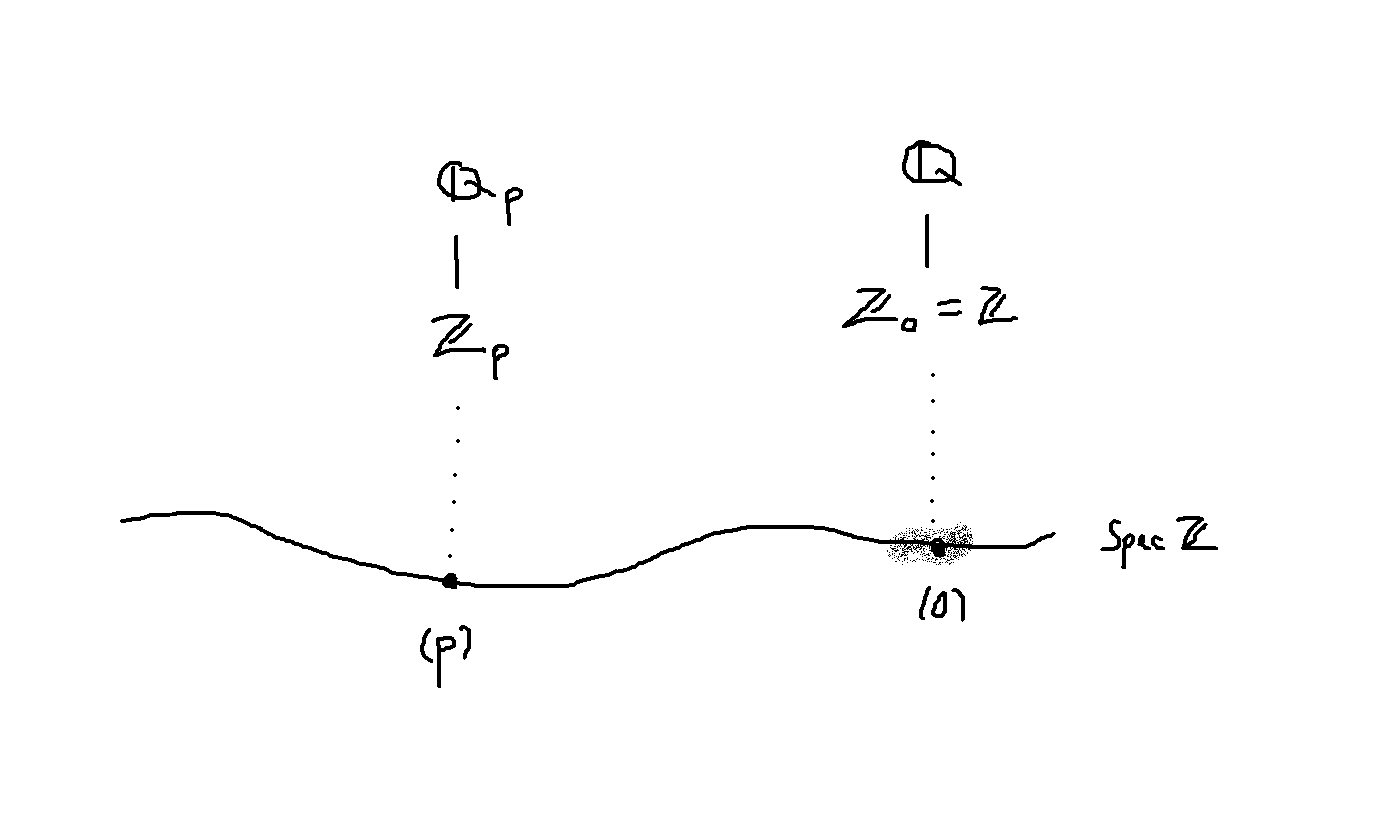
\includegraphics[width=\linewidth,height=\textheight,keepaspectratio]{Figures/places of Spec Z.png}
                        \caption{Places of $\Q$ (note that $(0)$ should be viewed as the generic place-at-infinity).}
                        \label{fig: places_of_Q}
                    \end{figure}
            \end{convention}
            
            \begin{proposition}[Local-global compatibility]
            
            \end{proposition}
                \begin{proof}
                    
                \end{proof}
            
            \begin{example}[Places of ramification of more general arithmetic schemes]
                Below are examples of arithmetic schemes, i.e. schemes over $\Spec \Z$, on which there are primes lying over those of $\Spec \Z$ where ramifications take place.
                    \begin{enumerate}
                        \item \textbf{(The prime spectrum of the ring of integers of a number field):} Consider the following setting:
                            $$
                                \begin{tikzcd}
                                	{\Q(\sqrt{d})} & {\Z[\sqrt{d}]} \\
                                	\Q & \Z
                                	\arrow[no head, from=2-1, to=1-1]
                                	\arrow[no head, from=2-2, to=1-2]
                                	\arrow[no head, from=1-1, to=1-2]
                                	\arrow[no head, from=2-1, to=2-2]
                                \end{tikzcd}
                            $$
                        wherein we are consider the quadratic extension $\Q(\sqrt{d})/\Q$ along with the induced integral extension of Dedekind domains $\Z[\sqrt{d}]/\Z$; particularly, let us pick a prime ideal $\p$ of $\Z$ (i.e. either the zero ideal or an ideal generated by a prime number $p$). Now, do the primes of $\Z[\sqrt{d}]$ indeed lie over those of $\Z$ ? First of all, we will need to see what the prime ideals of $\Z[\sqrt{d}]$ actually look like, and luckily, we can apply corollary \ref{coro: prime_splitting_finite_extensions} to do this:
                            \begin{enumerate}
                                \item Of course, the ideal $(0)\Z[\sqrt{d}]$ is just the zero ideal, and thus admits the trivial factorisation $(0) = (0)$. Because of this, let us only consider non-zero prime ideals of $\Z$ from now on.
                                \item Then, there are three cases, according to corollary \ref{coro: ramification_quadratic_fields}:
                                    \begin{enumerate}
                                        \item 
                                        \item
                                        \item
                                    \end{enumerate}
                            \end{enumerate}
                        \item \textbf{(A conic over $\Spec \Z$):}
                        \item \textbf{(The line with double origin over $\Spec \Z$):}
                    \end{enumerate}
                \end{example}
                
        \subsubsection{Unramfied morphisms}
            \begin{definition}[Unramified morphisms] \label{def: unramified_morphisms}
                A ring map is said to be \textbf{unramified} if it is of finite type and if the corresponding module of K\"ahler differentials is zero. 
            \end{definition}
            \begin{example}
                \noindent
                \begin{itemize}
                    \item \textbf{(\'Etale morphisms):} \'Etale morphisms (cf. definition \ref{def: etale_morphisms}) are trivially unramified. The converse statement is not necessarily true, since there are morphisms of finite type that are not of finite presentation, which is a necessary condition for \'etale-ness (or even just smoothness for that matter).
                    
                    As a concrete example, take any unramified finite extension $E/F$ (cf. definition \ref{def: ramification_indices}), and in the event that these fields have rings of integers (cf. example \ref{example: ring_of_integers}), the induced map:
                        $$\Spec E^{\circ} \to \Spec F^{\circ}$$
                    will also be unramified (in fact, they will be \'etale, since finite extensions come from finite presentations). As a result, for some fixed base scheme $S$, one can think of unramified morphisms $X \to S$ as coming from $S$-schemes $X$ such that preimages of points of $S$ consists merely of a single point. 
                    \item \textbf{(A counter example: non-\'etale smooth morphisms):} A smooth morphism of non-zero relative dimension can not be unramified, since its associated module of K\"ahler differential is not zero. 
                \end{itemize}
            \end{example}
            
            \begin{proposition}[Locality of ramification] \label{prop: locality_of_ramification}
                We say that 
            \end{proposition}
            
        \subsubsection{Extensions of discrete valuation rings}
            
        
        \subsubsection{Galois extensions and ramification}

\section{\'Etale cohomology for schemes: The Chosen One}
    \subsection{\'Etale morphisms} %\label{subsection: etale_morphisms}
        \begin{definition}[\'Etale morphisms] \label{def: etale_morphisms} \index{\'Etale-ness}
            An \'etale ring map is a smooth ring map whose cotangent complex is quasi-isomorphic to the zero complex. Equivalently, a ring homomorphism is \'etale if and only if it is smooth and of relative dimension $0$ (see proposition \ref{prop: smoothness_implies_almost_finiteness_of_cotangent_complex} for an explanation). 
        \end{definition}
        
        \begin{proposition}[The separable extension criterion for \'etale-ness] \label{prop: separable_criterion_for_etaleness} \index{\'Etale-ness! Separability Criterion}
            Let $\pi: F \to B$ be a ring map of finite presentation. Then, the following statements are equivalent:
                \begin{enumerate}
                    \item $\pi$ is \'etale.
                    \item The field extension $\kappa_{\pi^{-1}(\q)}/\kappa_{\q}$ of the residue field at $\pi^{-1}(\q) \in |\Spec k|$ over that at $\q \in |\Spec B|$ is separable (and necessarily finite, as \'etale maps are \textit{a priori} of finite presentation) for all $\q \in |\Spec B|$. Note that the extension $\kappa_{\pi^{-1}(\q)}/\kappa_{\q}$ exists thanks to the fact that the stalk map:
                        $$\calO_{\Spec F, \pi^{-1}(\q)} \to \calO_{\Spec B, \q}$$
                    which is actually just: 
                        $$F_{\pi^{-1}(\q)} \to B_{\q}$$
                    is required to be a local homomorphism between local rings.
                    \item If $F$ is a field, then $B$, when viewed as an $F$-vector space, can be written as a (necessarily finite) direct sum of (necessarily finite) separable extensions of $F$ (of course, this assertion is only equivalent to the other two in the event that they are considered with $F$ a field as well).
                \end{enumerate}
        \end{proposition}
            \begin{proof}
                This is trivial when $\chara \kappa_{\q} = 0$, as every extension in characteristic $0$ is \textit{a priori} separable (for a proof, please consult \cite[\href{https://stacks.math.columbia.edu/tag/030Q}{Tag 030Q}]{stacks} and \cite[\href{https://stacks.math.columbia.edu/tag/030N}{Tag 030N}]{stacks}). Thus, let us assume that:
                    $$\chara \kappa_{\q} = p$$
                for some prime $p$. Also, note that the extension $\kappa_{\pi^{-1}(\q)}/\kappa_{\q}$ decomposes into a separable part $\kappa_{\q}^{\sep}/\kappa_{\q}$ (with $\kappa_{\q}^{\sep}$ is the separable closure of $\kappa_{\q}$ inside $\kappa_{\pi^{-1}(\q)}$) and a purely inseparable part $\kappa_{\pi^{-1}(\q)}/\kappa_{\q}^{\sep}$ in the following manner \cite[\href{https://stacks.math.columbia.edu/tag/030K}{Tag 030K}]{stacks}:
                    $$
                        \begin{tikzcd}
                        	{\kappa_{\pi^{-1}(\q)}} \\
                        	{\kappa_{\q}^{\sep}} \\
                        	{\kappa_{\q}}
                        	\arrow[no head, from=3-1, to=2-1]
                        	\arrow[no head, from=2-1, to=1-1]
                        \end{tikzcd}
                    $$
                \begin{enumerate}
                    \item 
                        \begin{enumerate}
                            \item \textbf{(1 implies 2):} Suppose firstly that \textbf{1} holds, i.e. that $\pi: F \to B$ is \'etale. According to definition \ref{def: etale_morphisms}, this tells us that $B$ is a smooth $F$-algebra that is of relative dimension $0$; in other words, we can write $B$ as $\frac{F[x_1, ..., x_n]}{(f_1, ..., f_n)}$ for some natural number $n$. Now, fix an arbitrary prime ideal $\q \in \left|\Spec \frac{F[x_1, ..., x_n]}{(f_1, ..., f_n)}\right|$, which should be noted to be nothing but a prime of $F[x_1, ..., x_n]$ containing the ideal $(f_1, ..., f_n)$, and note that:
                                $$\left(\frac{F[x_1, ..., x_n]}{(f_1, ..., f_n)}\right)_{\q} \cong \frac{F[x_1, ..., x_n]_{\q}}{(f_1, ..., f_n)}$$
                            thanks to the fact that colimits commute. Now, let us suppose for the sake of deriving a contradiction, that $\kappa_{\pi^{-1}(\q)}/\kappa_{\q}$ is not a (finite) separable extension for our chosen prime $\q$, and observe that according to the preliminary discussion, this is the same as supposing that the purely inseparable extension $\kappa_{\pi^{-1}(\q)}/\kappa_{\q}^{\sep}$ is non-trivial. 
                            \item \textbf{(2 implies 1):} On the other hand, let us use \textbf{2} as our starting point. 
                        \end{enumerate}
                    \item 
                        \begin{enumerate}
                            \item \textbf{(2 implies 3):} Now, suppose that \textbf{2} is true and that $F$ is a field. Immediately, one sees that:
                                $$\kappa_{\pi^{-1}{\q}} \cong \calO_{\Spec F, \pi^{-1}(\q)} \cong F_{\pi^{-1}(\q)} \cong F_{(0)} \cong F$$ 
                            which means that $F/\kappa_{\q}$ is a (finite) separable extension for all primes $\q \in \left|\Spec B\right|$. Also, thanks to the hypothesis whereby $F$ is a field, one can write the finitely presented $F$-algebra $B$ as some finite direct some of copies of $F$ (since algebras are first and foremost modules, and modules over fields are vector spaces, which are \textit{a priori} all free). Thus, the \'etale $F$-algebra $B$, when viewed as a vector space over $F$, can written as a finite direct sum of the finite separable extension $F$ of $\kappa_{\q}$, for all $\q \in |\Spec B|$. In other words, \textbf{2} implies \textbf{3}. 
                            \item \textbf{(3 implies 2):} Conversely, suppose that \textbf{3} is true, specifically that:
                                $$B \cong F^{\oplus d}$$
                            for some natural number $d$, and suppose that the $F$-algebra of finite presentation $B$ is of the form $\frac{F[x_1, ..., x_N]}{(f_1, ..., f_n)}$, for some pair of natural numbers $n, N$. 
                        \end{enumerate}
                    Thus, we have managed to show that \textbf{1} is equivalent to \textbf{2}, and that \textbf{2} is in turn equivalent to \textbf{3}, and thus the three are jointly equivalent. 
                \end{enumerate}
            \end{proof}
        \begin{corollary}[Finite separable extensions are \'etale] \label{coro: finite_separable_extensions_are_etale}
            Let $k$ be a field and let $B$ be a $k$-algebra of finite presentation. According to proposition \ref{prop: separable_criterion_for_etaleness}, $B$ is \'etale over $k$ if and only if when it is viewed as a $k$-vector space, $B$ is a direct sum of copies of some finite separable extension $K$ over $k$. But $K$ itself is a $k$-algebra, and thus every finite and separable field extension is an \'etale ring map. In fact, it is even better: via the adjoint equivalence:
                $$
                    \begin{tikzcd}
                    	{{}^{k/}\Comm\Alg^{\op}} & {\Sch^{\aff}_{/\Spec k}}
                    	\arrow[""{name=0, anchor=center, inner sep=0}, "\Spec"', shift right=2, from=1-1, to=1-2]
                    	\arrow[""{name=1, anchor=center, inner sep=0}, "Gamma"', shift right=2, from=1-2, to=1-1]
                    	\arrow["\dashv"{anchor=center, rotate=-90}, draw=none, from=1, to=0]
                    \end{tikzcd}
                $$
            any non-empty collection of finite separable extension $\{k \to K_{\alpha}\}_{\alpha \in A}$ of some given ground field $k$ corresponds to an \'etale covering sieve $\{\Spec K_{\alpha} \to \Spec k\}_{\alpha}$ (because spectra of fields are singletons, the joint surjection of presheaves:
                $$
                    \begin{tikzcd}
                    	{\left(\coprod_{\alpha \in A} h_{\Spec K_{\alpha}}\right) \x_{h_{\Spec k}} \left(\coprod_{\alpha \in A} h_{\Spec K_{\alpha}}\right)} & {\coprod_{\alpha \in A} h_{\Spec K_{\alpha}}} & {h_{\Spec k}}
                    	\arrow["{\pr_2}"', shift right=2, from=1-1, to=1-2]
                    	\arrow["{\pr_1}", shift left=2, from=1-1, to=1-2]
                    	\arrow[dashed, from=1-2, to=1-3]
                    \end{tikzcd}
                $$
            exists for all non-empty indexing sets $A$). In turn, this implies something remarkable, which is that for all Galois extensions $K/k$ (which are necessarily separable by definition, and hence \'etale) and for all \textit{sheaves} $\calF$ on ${}^{k/}\Comm\Alg^{\op, \petit}_{\et}$ (we refer the reader to paragraph \ref{paragraph: etale_descent} for the descent theory along \'etale morphisms) we have via the fact that finite colimits (in this case, the orbit space ) commute with filtered limits that and the Fundamental Theorem of Galois Theory that:
                $$
                    \begin{aligned}
                        F(\Spec K)/Gal(K/k) & \cong \calF(\Spec E)/\left(\underset{E}{\lim} \Aut(E/k)\right)
                        \\
                        & \cong \underset{E}{\lim} \left(\calF(\Spec E)/\Aut(E/k)\right)
                        \\
                        & \cong \underset{E}{\lim} \left(\calF(\Spec k)/\Aut(E/k)\right)
                    \end{aligned}
                $$
            wherein the limit is the filtered limit taken over the poset of finite separable subextensions $E/k$ of $K/k$; also, note that:
                $$\calF(\Spec E) \cong \calF(\Spec k)$$
            for all finite separable extensions $E/k$ because sheaves satisfy descent, by definition.
        \end{corollary}
        \begin{remark}[Fibres over rational points of \'etale morphisms and inertia of primes] \label{remark: fibres_of_etale_maps_over_points}
            Let $k$ be a field and let $B$ be an \'etale $k$-algebra. From proposition \ref{prop: separable_criterion_for_etaleness}, we know that there exists a natural number $d$ such that:
                $$B \cong K^{\oplus d} \cong (k^{\oplus [K : k]})^{\oplus d} \cong k^{\oplus ([K : k] \cdot d)}$$
            as $k$-vector spaces, where $K/k$ is some finite separable extension. Then, thanks to the fact that direct sums of algebra objects in the category $k\Vect$ of $k$-vector spaces are merely products in the commutative algebra category ${}^{k/}\Comm\Alg$, and by employing the adjoint equivalence:
                $$
                    \begin{tikzcd}
                    	{{}^{k/}\Comm\Alg^{\op}} & {\Sch^{\aff}_{/\Spec k}}
                    	\arrow[""{name=0, anchor=center, inner sep=0}, "\Spec"', shift right=2, from=1-1, to=1-2]
                    	\arrow[""{name=1, anchor=center, inner sep=0}, "Gamma"', shift right=2, from=1-2, to=1-1]
                    	\arrow["\dashv"{anchor=center, rotate=-90}, draw=none, from=1, to=0]
                    \end{tikzcd}
                $$
            one gets:
                $$\Spec B \cong \Spec \prod_{i = 1}^d K \cong \coprod_{i = 1}^d \Spec K$$
            wherein the coproduct is taken in the category of locally ringed spaces over $\Spec k$, but lands in the category of affine schemes (also over $\Spec k$). Lastly, because spectra of fields are singletons, the \'etale $k$-algebra $B$ is nothing but a collection of $d$ disjoint points lying over the single point of $\Spec k$. 
            
            One implication of this is that given any scheme $X$ over $\Spec k$, its fibres over $k$-rational points $x \in X(k)$ are nothing but finite collections of points (even if the fibre is not affine, its affine patches would still necessarily be finite collections of points, as shown above, and thus the whole fibre would be so as well).
        \end{remark}

    \subsection{Galois cohomology}
        \subsubsection{Cohomology of profinite groups}
            Cohomology of profinite groups is nothing but group cohomology but for pro-objects in the category of finite groups (for us, cohomology shall always mean cohomology with abelian coefficients). Because of that, we shall pay less attention to the definition and general properties, and more on the special properties that cohomologies of profinite groups enjoy. By the end of it, we shall apply what we know to Galois groups, which are profinite thanks to the Fundamental Theorem of Galois Theory. 
            
            \paragraph{Group cohomology}
                \begin{convention}
                    \noindent
                    \begin{itemize}
                        \item Throughout, we shall work with a sheaf topos $\E$ in which the category of internal abelian groups $\Ab(\E)$ has enough projectives (for instance, one can consider $\E \cong \Sets$ or the \'etale topos over any qcqs scheme). This essentially just means that we are assuming that the internal logic of $\E$ supports the Axiom of Choice (or more minimally, the Axiom of Presentation). 
                        
                        In particular, fix an abelian group $A \in \Ab(\E)$.
                        \item Additionally, fix a group object $G \in Grp(\E)$. Its group ring shall be denoted by $\Z[G]$ (which is not an abuse of notation, since a natural number object exists in $\E$, allowing us to define an integer object $\Z$ as the group completion of the monoid $\N$; alternatively, one can think of $\Z$ as the monoidal unit of $\Ab(\E)$); recall that this ring object is defined via the following forgetful-free adjunction, whose existence we shall let the reader prove as an exercise\footnote{Recall that $\Ring(\E)$ is the category of monoids internal to the symmetric monoidal category $\Ab(\E)$.}:
                            $$
                                \begin{tikzcd}
                                	{\Ring(\E)} & {\Grp(\E)}
                                	\arrow[""{name=0, anchor=center, inner sep=0}, "\oblv"', shift right=2, from=1-1, to=1-2]
                                	\arrow[""{name=1, anchor=center, inner sep=0}, "{\Z[-]}"', shift right=2, from=1-2, to=1-1]
                                	\arrow["\dashv"{anchor=center, rotate=-90}, draw=none, from=1, to=0]
                                \end{tikzcd}
                            $$
                            
                        We shall also want a $G$-action on $A$, which would make $A$ a $\Z[G]$-module.
                    \end{itemize}
                \end{convention}
                
                \begin{definition}[Group cohomologies] \label{def: group_cohomologies}
                    The $n^{th}$ cohomology group of $G$ with coefficient in $A$ is defined as:
                        $$H^n(G, A) \cong \Ext^n_{\Z[G]}(\Z, A)$$
                    where we view $\Z$ as trivial $G$-representation on the right-hand side. 
                \end{definition}
                \begin{remark}
                    It is not hard to see via induction on the cohomological dimension $n \in \N$ that $H^n(G, A)$ (as in definition \ref{def: group_cohomologies}) actually has a $k$-module structure.
                \end{remark}
                
                Let us now attempt to compute cohomologies of groups in low dimensions (namely, $n = 0, 1, 2$) as well as give meaning to these spaces, which we shall do using free (or at worst, projective) resolutions of the trivial $\Z[G]$-module $\Z$.
                \begin{proposition}[Low-dimensional cohomologies of groups] \label{prop: low_dimensional_cohomologies_of_groups}
                    One has the following interpretations of the low-dimensional cohomologies of $G$ with coeffcients in $A$:
                    \begin{enumerate}
                        \item \textbf{($n = 0$: Invariants):}
                            $$H^0(G, A) \cong A^G$$
                        with $A^G$ denoting the space of $G$-fixed point of $A$.
                        \item \textbf{($n = 1$: Torsors):} 
                        \item \textbf{($n = 2$: Extensions):} 
                            $$H^2(G, A) \cong \{\text{extensions of $G$ by $A$}\}$$
                    \end{enumerate}
                \end{proposition}
                    \begin{proof}
                        \noindent
                        \begin{enumerate}
                            \item \textbf{($n = 0$: Invariants):}
                            \item \textbf{($n = 1$: Torsors):}
                            \item \textbf{($n = 2$: Extensions):}
                        \end{enumerate}
                    \end{proof}
                \begin{example}
                                
                \end{example}
            
            \paragraph{Properties of cohomologies of profinite groups}
        
        \subsubsection{Iwasawa theory}
        
    \subsection{\'Etale fundamental groups}
        \subsubsection{Construction of \'etale fundamental groups}
            \'Etale fundamental groups of schemes as in \cite[Expos\'e V]{SGA1} are constructed using so-called \textbf{finite Galois categories}: in particular, for any fixed scheme $X$, the category of finite \'etale $X$-schemes is an instance of a finite Galois category, for whom the fundamental group is the group of natural automorphisms of the \textbf{fibre functor} based at a geometric point $\bar{x} \in X$:
                $$\Fib_{\bar{x}}: (\Sch_{/X})_{\fet} \to \Fin\Sets$$
                $$Y \mapsto Y(\bar{x})$$
            Below shall be a brief discussion of the construction (remark \ref{remark: finite_etale_schemes}) and key properties of \'etale fundamental groups of schemes (propositions \ref{prop: etale_fundamental_groups_do_not_depend_on_base_points} and \ref{prop: etale_homotopy_exact_sequence}), accompanied by certain relevant examples (cf. examples \ref{example: etale_fundamental_group_of_a_field} and \ref{example: etale_fundamental_group_of_a_curve}). 
            
            We begin with the notion of finite Galois categories. Heuristically speaking, these are categories which are equivalent to $\pi\-\Fin\Sets$, the category of finite sets with actions of some profinite group $\pi$, which as we shall see, serves as the \say{fundamental group} of its associated finite Galois category. Due to this phenomenon, the fundamental group of a Galois category serves the same purpose as the classical fundamental groups of topological spaces, that being as a topological invariant. 
            \begin{definition}[Finite Galois categories] \label{def: finite_galois_categories}
                \noindent
                \begin{itemize}
                    \item \textbf{(Finite Galois categories):} A \textbf{finite Galois category} is defined via the data contained in a pair $(\calG, F)$ consisting of:
                    \begin{itemize}
                        \item a \textit{finitely complete and finitely cocomplete} small category $\calG$, wherein objects can all be written as finite coproducts of \textit{connected} objects\footnote{Objects $Y \in \calG$ such that the copresheaf $h^Y: \calG \to \Sets$ preserves all coproducts.}, and
                        \item a \textit{pro-representable} functor $F: \calG \to \Fin\Sets$, called the \textbf{fibre functor}, which we shall require to be reflect and preserve all finite limits and finite colimits.
                    \end{itemize}
                    \item \textbf{(Galois objects):} An object $Y$ of a finite Galois category $\calG$ is a \textbf{Galois object} if and only if $Y/\Aut(Y)$ is terminal as an object of $\calG$ (which exists as $\calG$ is finitely complete by definition).
                    \item \textbf{(Galois functors):} A \textbf{Galois functor} is an exact functor $\Phi: \calG \to \calG'$ between finite Galois categories $(\calG, F), (\calG', F')$ which preserves connected objects and commute with the fibre functors in the following manner:
                        $$
                            \begin{tikzcd}
                            	\calG && {\calG'} \\
                            	& \Fin\Sets
                            	\arrow["F"', from=1-1, to=2-2]
                            	\arrow["{F'}", from=1-3, to=2-2]
                            	\arrow["\Phi", from=1-1, to=1-3]
                            \end{tikzcd}
                        $$
                \end{itemize}
            \end{definition}
            \begin{remark}
                What we refer to as \say{finite Galois categories} here are simply \say{Galois categories} in both \cite[Expos\'e V]{SGA1} and \cite[\href{https://stacks.math.columbia.edu/tag/0BMQ}{Tag 0BMQ}]{stacks}. We have done this in order to highlight the relationship between our \say{finite Galois categories} and the \say{infinite Galois categories} from \cite[Section 7]{bhatt_scholze_2014_pro_etale} (cf. definition \ref{def: infinite_galois_categories}).
            \end{remark}
            
            \begin{lemma}[Galois covers of connected objects] \label{lemma: galois_covers_of_connected_objects}
                \cite[\href{https://stacks.math.columbia.edu/tag/0BN2}{Tag 0BN2}]{stacks} Let $(\calG, F)$ be a finite Galois category and let $Y$ be a connected object. Then, there exits a Galois object $\tilde{Y}$ and a morphism $\tilde{p}: \tilde{Y} \to Y$.
            \end{lemma} 
            \begin{corollary}[Cofiltered diagrams of Galois objects] \label{coro: cofiltered_diagrams_of_Galois_objects_in_a_finite_Galois_category}
                If $(\calG, F)$ is a finite Galois category then the full subcategory of Galois objects is cofiltered (cf. \cite[\href{https://stacks.math.columbia.edu/tag/00D3}{Tag 00D3}]{stacks}).
            \end{corollary}
            \begin{remark}
                Lemma \ref{lemma: galois_covers_of_connected_objects} ought to be thought of as a vast generalisation of the fact that every separable extension admits a Galois closure (or perhaps more fundamentally, the fact that every subgroup admits a normal closure). Why this is the case can be seen using the Galois Correspondence for fields (or alternatively, the Galois Correspondence for covering spaces; cf. \cite[Theorem 1.38]{hatcher2002algebraic}): if $L/K$ is a Galois extension then subgroups $H \leq \Gal(L/K)$ are normal if and only if the corresponding subextension is normal and likewise, if $Y \to Y' \to X$ is a tower of connected coverings then $\Aut(Y'/X)$ is a normal subgroup of $\Aut(Y/X)$ if and only if $Y' \to X$ is Galois\footnote{We have omitted certain mild technical assumptions here. For a more detailed account, see \cite[Section 1.3]{hatcher2002algebraic}.}. 
            \end{remark}
            \begin{lemma}[Morphisms between connected objects are epic] \label{lemma: morphisms_between_connected_objects_are_epic}
                In any finite Galois category, morphisms between connected objects are epimorphisms and vice versa, the codomain of an epimorphism whose domain is connected is also connected.
            \end{lemma}
                \begin{proof}
                    See \cite[\href{https://stacks.math.columbia.edu/tag/0BN0}{Tag 0BN0}]{stacks} and \cite[Proposition 3.5]{nlab:connected_objects}.
                \end{proof}
            \begin{proposition}[Fibre functors of finite Galois categories are pro-represented by Galois objects] \label{prop: fibre_functors_of_finite_galois_categories_are_pro_represented_by_galois_objects}
                \cite[\href{https://stacks.math.columbia.edu/tag/0BN3}{Tag 0BN3}]{stacks} Let $(\calG, F)$ be a finite Galois category. Then, the fibre functor $F$ is pro-represented by any cofinal diagram in the full subcategory spanned by Galois objects of $\calG$.
            \end{proposition}
            \begin{corollary}[There is only one fibre functor!] \label{coro: only_one_fibre_functor_on_a_finite_galois_category}
                Let $\calG$ be a finite Galois category and let $F, F'$ be fibre functors thereon. Then $F \cong F'$, as they are pro-represented by cofinal pro-object of $\calG$.
            \end{corollary}
            
            \begin{definition}[Fundamental groups of finite Galois categories] \label{def: fundamental_groups_of_finite_galois_categories}
                The \textbf{fundamental group} of a given finite Galois category $(\calG, F)$, denoted by $\pi_1(\calG, F)$, is defined to be $\Aut(F)$.
            \end{definition}
            
            \begin{definition}[Profinite completions of groups] \label{def: profinite_completions_of_groups}
                The \textbf{profinite completion} of a topological group $G$, denoted by $\hat{G}$, is the limit in $\Sets$ of the cofiltered diagram $\{G/N\}_{\text{$N \leq G$ open, normal, finite-index}}$. 
            \end{definition}
            \begin{proposition}[Finite Galois categories of equivariant finite sets] \label{prop: finite_galois_categories_of_equivariant_finite_sets}
                Let $G$ be a topological group and let $\oblv_G: G\-\Fin\Sets \to \Fin\Sets$ denote the forgetful functor going from the category of finite sets with continuous actions of $G$, to that of finite sets. Then there is an isomorphism of profinite groups $\Aut(\oblv_G) \cong \hat{G}$. Furthermore, $G\-\Fin\Sets$ is a finite Galois category if and only if $G$ is a profinite group. 
            \end{proposition}
                \begin{proof}
                    Combine \cite[IV.2.4 et IV.2.7]{sga4} with \cite[\href{https://stacks.math.columbia.edu/tag/0BMU}{Tag 0BMU}]{stacks}.
                \end{proof}
                
            \begin{lemma}[Endomorphisms on Galois objects are automorphisms] \label{lemma: endomorphisms_on_galois_objects_of_finite_galois_categories_are_automorphisms}
                \cite[pp. 100]{SGA1} All endomorphisms on a Galois object of a finite Galois category are automorphisms.
            \end{lemma}
            \begin{proposition}[Fundamental groups of finite Galois categories are profinite] \label{prop: fundamental_groups_of_finite_galois_categories_are_profinite}
                The fundamental group of any finite Galois category is profinite. In fact, given a finite Galois category $(\calG, F)$, its fundamental group arises as the limit of the cofiltered diagram $\{\Aut(F(Y_i))\}_{i \in \calI}$, where $\calI$ is any cofinal diagram of Galois objects in $\calG$.
            \end{proposition}
                \begin{proof}
                    Using proposition \ref{prop: fibre_functors_of_finite_galois_categories_are_pro_represented_by_galois_objects}, suppose that $F \cong \underset{i \in \calI}{\colim} h^{Y_i}$, with $\{Y_i\}_{i \in \calI}$ being a cofinal diagram of Galois objects. From this, and from the fact that all fibre functors on the same finite Galois category are isomorphic (cf. corollary \ref{coro: only_one_fibre_functor_on_a_finite_galois_category}), one sees that:
                        $$\pi_1(\calG, F) \cong \Aut(F) \cong \Nat(F, F) \cong \underset{i \in \calI}{\lim} \Nat(h^{Y_i}, h^{Y_i}) \cong \underset{i \in \calI}{\lim} \calG(Y_i, Y_i)$$
                    Since all endomorphisms on a Galois object of a finite Galois category are automorphisms (cf. lemma \ref{lemma: endomorphisms_on_galois_objects_of_finite_galois_categories_are_automorphisms}), the above tells us that $\pi_1(\calG, F) \cong \underset{i \in \calI}{\lim} \Aut(Y_i)$. Finally, because $F$ reflects isomorphisms by definition, we have an isomorphism $\Aut(Y_i) \cong \Aut(F(Y_i))$ for all $Y_i$; this implies that $\pi_1(\calG, F) \cong \underset{i \in \calI}{\lim} \Aut(F(Y_i))$, which concludes the proof.
                \end{proof}
            \begin{corollary}[Fundamental groups of finite Galois categories act transitively on connected objects] \label{coro: fundamental_groups_of_finite_galois_categories_act_transitively_on_connected_objects}
                Let $(\calG, F)$ be a finite Galois category. Then, $\pi_1(\calG, F)$ acts\footnote{See remark \ref{remark: action_of_fundamental_groups_on_fibres_finite_galois_categories} for an explanation of why such actions even existed in the first place.} transitively and continuously on $F(Y)$ whenever $Y$ is connected. Furthermore, the functor $F$ preserves connectedness of objects. 
            \end{corollary}
            
            \begin{definition}[The compact-open topology] \label{def: the_compact_open_topology}
                Let $X, Y$ be topological spaces and for all $K \subseteq X$ closed (respectively, compact) and all $V \subseteq Y$ open, set $\<K, U\> := \{\varphi \in \Maps(X, Y) \mid \varphi(K) \subseteq U\}$. Then, it can be shown that the collection of sets $\<K, U\>$ as above generates a topology on $\Maps(X, Y)$, which is known as the \textbf{closed-open} (respectively, \textbf{compact-open}) topology.
            \end{definition}
            \begin{lemma}[The compact-open topology on automorphism groups] \label{lemma: the_compact_open_topology_on_automorphism_groups}
                \cite[Theorem 3.5.2 and Corollary 3.5.3]{topological_groups_and_related_structures} Let $X$ be a normal topological space. Then, $\Aut(X)$ will become a topological group if endowed with the subspace topology induced by the closed-open topology on $\Maps(X, X)$. If $X$ is furthermore a compact Hausdorff space then the closed-open and compact-open topologies on $\Aut(X)$ will coincide.
            \end{lemma}
            \begin{example}[The compact-open topology on automorphism groups of sets] \label{example: the_compact_open_topology_on_automorphism_groups_of_sets}
                \noindent
                \begin{itemize}
                    \item \textbf{(Discrete sets):} \cite[\href{https://stacks.math.columbia.edu/tag/0BMC}{Tag 0BMC}]{stacks} If $S$ is a set equipped with the discrete topology, then $\Aut(S)$ shall naturally be a topological group if equipped with either the closed-open topology or the compact-open topology. However, because discrete sets are compact if and only if they are finite, the two topologies can only coincide in that situation.
                    \item \textbf{(Profinite sets):} If $S$ is a profinite set (hence compact and Hausdorff; cf. \cite[\href{https://stacks.math.columbia.edu/tag/08ZY}{Tag 08ZY}]{stacks}) then $\Aut(S)$ shall be the same topological group, regardless of whether it is equipped with the or closed-open topology or the compact-open topology. 
                \end{itemize}
            \end{example}
            \begin{remark}[Action of fundamental groups on fibres] \label{remark: action_of_fundamental_groups_on_fibres_finite_galois_categories}
                Let $(\calG, F)$ be a finite Galois category. First of all, note that because such categories are small and because the category of groups has all (small) products, the product $\prod_{Y \in \Ob(\calG)} \Aut(F(Y))$ is well-defined as a (discrete) group. Now, if we were to endow each $\Aut(F(Y))$ with the subspace topology\footnote{Which is discrete when $F(Y)$ (or rather, $\Aut(F(Y))$) is finite (cf. example \ref{example: the_compact_open_topology_on_automorphism_groups_of_sets}).} inherited from $\Maps(F(X), F(X))$ with the compact-open topology, and then $\pi_1(\calG, F) := \Aut(F)$ with the subspace topology inherited from the product topology on $\prod_{Y \in \Ob(\calG)} \Aut(F(Y))$, then $\pi_1(\calG, F)$ shall act \textit{continuously} on the sets $F(X)$, as seen from the following commutative diagram of topological groups and continuous homomorphisms:
                    $$
                        \begin{tikzcd}
                        	{\pi_1(\calG, F)} & {\prod_{Y \in \Ob(\calG)} \Aut(F(Y))} \\
                        	& {\Aut(F(Y))}
                        	\arrow[tail, from=1-1, to=1-2]
                        	\arrow[two heads, from=1-2, to=2-2]
                        	\arrow[dashed, from=1-1, to=2-2]
                        \end{tikzcd}
                    $$
                As such, the fibre functor $F: \calG \to \Fin\Sets$ factors in the following manner through the category $\pi_1(\calG, F)\-\Fin\Sets$ of finite sets operated on continuously by $\pi_1(\calG, F)$:
                    $$
                        \begin{tikzcd}
                        	\calG && {\pi_1(\calG, F)\-\Fin\Sets} \\
                        	& \Fin\Sets
                        	\arrow[dashed, from=1-1, to=1-3]
                        	\arrow["F"', from=1-1, to=2-2]
                        	\arrow["{\oblv_{\pi_1(\calG, F)}}", from=1-3, to=2-2]
                        \end{tikzcd}
                    $$
                wherein $\oblv_{\pi_1(\calG, F)}: \pi_1(\calG, F)\-\Fin\Sets \to \Fin\Sets$ denotes the forgetful functor. Eventually, we will show that this factorisation is actually a Galois equivalence between $\calG$ and $\pi_1(\calG, F)\-\Fin\Sets$ (see theorem \ref{theorem: finite_categorical_galois_correspondence} below).
            \end{remark}
            \begin{theorem}[The Finite Galois Correspondence] \label{theorem: finite_categorical_galois_correspondence}
                \cite[\href{https://stacks.math.columbia.edu/tag/0BN4}{Tag 0BN4}]{stacks} For any finite Galois category $(\calG, F)$, the functor $F: \calG \to \pi_1(\calG, F)\-\Fin\Sets$ is a Galois equivalence (we equip the latter with the forgetful functor to $\Fin\Sets$).
            \end{theorem}
                \begin{proof}
                    This is essentially the same as the proof of theorem \ref{theorem: infinite_categorical_galois_correspondence}. We shall leave the imposing of the relevant finiteness conditions as in definition \ref{def: finite_galois_categories} up to the reader. 
                \end{proof}
            
            Now, the \'etale fundamental group is literally the fundamental group of a Galois category by construction. Namely, it is the fundamental group of the finite Galois category of pointed schemes that are finite \'etale over a pointed base scheme $(X, \bar{x})$ (cf. remark \ref{remark: finite_etale_schemes}). This, however, is not the only interesting feature that the \'etale fundamental group displays; one of the main reason why Grothendieck's \'etale fundamental group gained attention in the first place is that by taking the \'etale fundamental group of an algebraic variety, one actually obtains the absolute Galois of the global function field of said variety. As such, the \'etale fundamental group is a great tool that we can make use of in order to understand Galois groups; in fact, even the use of finite \'etale morphisms has a very concrete field-theoretic reason (cf. \cite[\href{https://stacks.math.columbia.edu/tag/00U3}{Tag 00U3}]{stacks}).
            
            Let us also note that because any topological space with a generic point is contractible \textit{a priori}, and since most interesting schemes (such as varieties) are integral and hence have generic points\footnote{This is more or less due to the fact that the zero ideal is prime in integral domains. For more details, see \cite[\href{https://stacks.math.columbia.edu/tag/01IS}{Tag 01IS}]{stacks-project}.}, the usual topological fundamental group is very unlikely to be able to distinguish the underlying topological spaces of two different schemes. Furthermore, because schemes are actually determined by their structure sheaves as opposed to their underlying topological spaces (e.g. if $\Nil(R)$ denotes the nilradical of a commutative ring then $\Spec R$ and $\Spec R/\Nil(R)$ will be non-isomorphic schemes whose underlying topological spaces are homeomorphic), we should not expect the topological fundamental group to be able to tell two schemes apart from one another. This is not to mention that in most cases, the underlying topological space of a scheme is not path-connected, so a fundamental group defined as the group of homotopy equivalence class of loops would not have made much sense.
            \begin{remark}[Finite-\'etale schemes] \label{remark: finite_etale_schemes}
                For any given by scheme $X$, the small category $(\Sch_{/X})_{\fet}$ of finite-\'etale $X$-schemes is a category wherein:
                    \begin{itemize}
                        \item all finite limits and all finite colimits exist, and
                        \item all objects can be written as a (possibly empty) finite coproduct of connected objects, which happen to be schemes that are \'etale over $X$.  
                    \end{itemize}
                (for a detailed proof, see \cite[\href{https://stacks.math.columbia.edu/tag/0BN9}{Tag 0BN9}]{stacks}) so should we be able to define a fibre functor $(\Sch_{/X})_{\fet} \to \Fin\Sets$, we will have succeeded in putting a finite Galois category structure on $(\Sch_{/X})_{\fet}$. As a matter of fact, such a well-defined fibre functor has good reasons to exist: it is an easy consequence of \cite[\href{https://stacks.math.columbia.edu/tag/00U3}{Tag 00U3}]{stacks} that for any fixed geometric point $\bar{x} \in X$ (corresponding to an algebraic closure\footnote{Certain sources consider geometric points to correspond to separable closures. For us, however, geometric points are algebraically closed fields $K$ so that $\Spec K$ be a Galois object of $(\Sch_{/\Spec K})_{\fet}$. In practice this choice usually does not matter, since we will mostly work over perfect field, and separable closures of perfect fields are algebraically closed.} $\bar{\kappa}_x$ of the residue field of $x \in X$), one has:
                    $$(\Spec \bar{\kappa}_x)_{\fet} \cong \Fin\Sets$$
                (the forward direct simply involves taking the underlying set, and the inverse functors is given by $I \mapsto \coprod_{i = 1}^{|I|} \Spec \bar{\kappa}_x$) and so for any $k$-scheme $X$, one has the following canonical defined functor:
                    $$(\Sch_{/X})_{\fet} \to (\Sch_{/\Spec \bar{\kappa}_x})$$
                    $$Y \mapsto Y_{\bar{x}}$$
                where $Y_{\bar{x}} \cong Y \x_X \Spec \bar{\kappa}_x$; one can then take the underlying set of $Y_{\bar{x}}$ to get the following trivially left-exact\footnote{... and hence pro-representable (cf. \cite[Proposition 3.1]{grothendieck_fga_2}).} functor:
                    $$\Fib_{\bar{x}}: (\Sch_{/X})_{\fet} \to \Fin\Sets$$
                    $$Y \mapsto |Y_{\bar{x}}|$$
                We should also verify that the sets $|Y_{\bar{x}}|$ are indeed finite. To this end, let us first apply the fact that pullbacks of \'etale morphisms are \'etale to see that if $Y$ is affine over $X$ then $Y_{\bar{x}}$ will have to be the spectrum of an \'etale $\bar{\kappa}_x$-algebra; however, according to \cite[\href{https://stacks.math.columbia.edu/tag/00U3}{Tag 00U3}]{stacks}, this means that $Y_{\bar{x}} \cong \Spec (\bar{\kappa}_x)^{\oplus N}$ for some finite $N$. The locality of \'etale-ness and the finiteness of $Y$ as an $X$-scheme then tells us that in general, $Y_{\bar{x}}$ must be a finite disjoint union of affine schemes of the form $\Spec (\bar{\kappa}_x)^{\oplus N}$, meaning that $Y_{\bar{x}} \cong \Spec (\bar{\kappa}_x)^{\oplus N'}$ for some finite $N'$. The set $|Y_{\bar{x}}|$ is therefore always finite. One also sees that an immediate consequence of this proof is that $\Fib_{\bar{x}}$ necessarily \textit{reflects isomorphisms} and is \textit{right-exact}. 
            \end{remark}
            
            The discussion above allows us to make the following important definition.
            \begin{definition}[\'Etale fundamental groups of schemes] \label{def: etale_fundamental_groups_of_schemes}
                For any scheme $X$ with a fixed geometric point $\bar{x}$, the pair $((\Sch_{/X})_{\fet}, \Fib_{\bar{x}})$ as in remark \ref{remark: finite_etale_schemes} defines a finite Galois category in the sense of definition \ref{def: finite_galois_categories}. Its fundamental group is commonly denoted by $\pi_1(X_{\fet}, \bar{x})$ and called the \textbf{\'etale fundamental group} of $X$ based at $\bar{x}$.
            \end{definition}
            
            We can then apply theorem \ref{theorem: finite_categorical_galois_correspondence} directly to get the following topological characterisation of connected schemes via their \'etale fundamental groups.
            \begin{theorem}[The Geometric Galois Correspondence] \label{theorem: geometric_galois_correspondence}
                For $(X, \bar{x})$ a pointed connected scheme, the functor $\Fib_{\bar{x}}: (\Sch_{/X})_{\fet} \to \Fin\Sets$ as in remark \ref{remark: finite_etale_schemes} above is a Galois equivalence of finite Galois categories. 
            \end{theorem}
            \begin{corollary}
                Should $H$ be a finite-index (hence open, since $\pi_1(X_{\fet}, \bar{x})$ is profinite \textit{a priori}; cf. proposition \ref{prop: fundamental_groups_of_finite_galois_categories_are_profinite}) normal subgroup of $\pi_1(X_{\fet}, \bar{x})$ and $(X^H, \bar{x}^H)$ be the corresponding Galois $X$-scheme with a choice of base point $\bar{x}^H$ lying over $\bar{x}$, then $\pi_1(X^H_{\fet}, \bar{x}^H) \cong H$. In fact, for any connected pointed scheme $(X, \bar{x})$, there is an equivalence of categories:
                    $$\{\text{Finite \'etale $X$-schemes $Y$ with base points $\bar{y}$ lying over $\bar{x}$}\}$$
                    $$\cong$$
                    $$\{\text{Finite-index subgroups of $\pi_1(X_{\fet}, \bar{x})$}\}$$
                which restricts down to:
                    $$\{\text{Finite \'etale Galois $X$-schemes $Y$ with base points $\bar{y}$ lying over $\bar{x}$}\}$$
                    $$\cong$$
                    $$\{\text{Finite-index \textit{normal} subgroups of $\pi_1(X_{\fet}, \bar{x})$}\}$$
            \end{corollary}
            \begin{example}[The \'etale fundamental group of a field] \label{example: etale_fundamental_group_of_a_field}
                As a sanity check, note that if $K$ is a field then finite-\'etale Galois schemes over $\Spec K$ shall be of the form $\Spec L \to \Spec K$, where $L/K$ is a finite Galois extension, and as a consequence, there are the following equivalences of categories\footnote{In fact, these categories are lattices with meets being intersections of fields/subgroups and joins being the constructions of composite fields/subgroups.}, which demonstrate that theorem \ref{theorem: geometric_galois_correspondence} directly generalises the classical Galois Correspondence:
                    $$\{\text{Finite-index normal subgroups of $\pi_1((\Spec K)_{\fet})$}\}$$
                    $$\cong$$
                    $$\{\text{Finite \'etale Galois schemes over $\Spec K$}\}$$
                    $$\cong$$
                    $$\{\text{Finite Galois extensions of $K$}\}^{\op}$$
                    $$\cong$$
                    $$\{\text{Finite-index normal subgroups of $\Gal(\bar{K}/K)$}\}$$
            \end{example}
            \begin{example}[The \'etale fundamental group of a curve] \label{example: etale_fundamental_group_of_a_curve}
                \noindent
                \begin{itemize}
                    \item \textbf{(Projective line):} Let $k$ be a field. If $X$ is a connected non-singular projective curve over $\Spec k$ with function field $K$, then there is a canonical equivalence between the categories of finite Galois extensions of $K$ and finite \'etale Galois $X$-schemes, which are precisely dominant rational maps whose associated function field extensions are Galois thanks to proposition \ref{prop: curves_and_function_fields}. Through this, it is easy to see that:
                        $$\pi_1(X_{\fet}) \cong \Gal(\bar{K}/K)$$
                    For instance, we have:
                        $$\pi_1((\P^1_k)_{\fet}) \cong \Gal(\bar{k}/k)$$
                    (since the function field of $\P^1_k$ is $k(t)$), which tells us that $\P^1_k$ is simply \'etale-connected if and only if $k$ is algebraically closed (since $\Gal(\bar{k}/k)$ is \textit{a fortiori} trivial in that case). 
                    \item \textbf{(Elliptic curves):} Another interesting case that one might wish to consider is that of elliptic curves; for the sake of simplicity, let us work with an elliptic curve $E$ over an algebraically closed field $k$ of characteristic $0$. First of all, because $k$ is algebraically closed, every $k$-rational point $x \in E(k)$ is automatically geometric; therefore, we might as well work with $x = 0$. Now, it can be shown without too much difficulty (cf. \cite[Proposition 5.11]{kundu_etale_fundamental_group_of_elliptic_curves}) that every scheme finite \'etale over an elliptic curve over any field is automatically Galois. Together with the definition of $\pi_1(E_{\fet})$, this implies that for any cofinal diagram $\{Y_i\}_{i \in \calI}$ in $(\Sch_{/E})_{\fet}$, one has:
                        $$\pi_1(E_{\fet}) \cong \underset{i \in \calI}{\lim} \Aut(F_0(Y_i)) \cong \underset{i \in \calI}{\lim} \Aut(|(Y_i)_0|)$$
                    Luckily, there is a canonical choice of such a cofinal diagram, namely $\{E[n]\}_{n \in \N}$ (cf. \cite[Proposition 3.8]{kundu_etale_fundamental_group_of_elliptic_curves}), which are nothing but the fibres over $0 \in E(k)$ (i.e. kernels) of the $n$-torsion maps $[n]: E \to E$ (this is why we chose the base point $x = 0$). It is well-known that $\Aut(|E[n]|) \cong (\Z/n\Z)^{\oplus 2}$, so by taking the limit, one obtains:
                        $$\pi_1(E_{\fet}) \cong \hat{\Z}^{\oplus 2}$$
                    Elliptic curves over (algebraically closed) fields of positive characteristics $p_0$ behave somewhat differently, but it is also difficult to compute their \'etale fundamental groups (provided). If $E$ is supersingular (i.e. if the $p_0$-torsion map $[p_0]: E \to E$ has trivial kernel) then one has the following description of the \'etale fundamental group of $E$ (cf. \cite[Proposition 5.13]{kundu_etale_fundamental_group_of_elliptic_curves}):
                        $$\pi_1(E_{\fet}) \cong \bigoplus_{(p) \in |\Spec \Z| \setminus \{(0), (p_0)\}} \Z_p^{\oplus 2}$$
                    and otherwise, if $E$ is an ordinary elliptic curve, one has the following (cf. \cite[Proposition 5.14]{kundu_etale_fundamental_group_of_elliptic_curves}):
                        $$\pi_1(E_{\fet}) \cong \Z_{p_0} \oplus \bigoplus_{(p) \in |\Spec \Z| \setminus \{(0), (p_0)\}} \Z_p^{\oplus 2}$$
                \end{itemize}
            \end{example}
        
        \subsubsection{Properties of \'etale fundamental groups}
            Now, let us make sure that the \'etale fundamental group $\pi_1(X_{\fet}, \bar{x})$ as defined in definition \ref{def: etale_fundamental_groups_of_schemes} is meaningful as a formal construction. Namely, we would like to know the behaviours of $\pi_1(X_{\fet}, \bar{x})$ when we change the base point and when we base-change (cf. proposition \ref{prop: etale_fundamental_groups_do_not_depend_on_base_points}), as well as whether or not \'etale fibrations induce homotopy exact sequences of fundamental groups (cf. proposition \ref{prop: etale_homotopy_exact_sequence}). 
            \begin{proposition}[\'Etale fundamental group do not depend on base points] \label{prop: etale_fundamental_groups_do_not_depend_on_base_points}
                \cite[\href{https://stacks.math.columbia.edu/tag/0BQA}{Tag 0BQA}]{stacks} Let $f: Y \to X$ be a morphism of connected qcqs\footnote{quasi-compact and quasi-separated} schemes such that the base change functor $X' \mapsto X' \x_X Y$ is an equivalence of Galois categories between $(\Sch_{/X})_{\fet}$ and $(\Sch_{/Y})_{\fet}$. Then, for any choice of geometric points $\bar{x} \in X$ and $\bar{y} \in Y$, one has the following isomorphism of \'etale fundamental groups $\pi_1(X_{\fet}, \bar{x}) \cong \pi_1(Y_{\fet}, \bar{y})$.
            \end{proposition}
            \begin{corollary}[Uniqueness of \'etale fundamental groups] \label{coro: etale_fundamental_group_uniqueness}
                For any connected qcqs scheme $X$ and any pair of possibly distinct geometric points $\bar{x}, \bar{x}' \in X$, one has any isomorphism of \'etale fundamental groups $\pi_1(X_{\fet}, \bar{x}) \cong \pi_1(X_{\fet}, \bar{x}')$, and therefore it makes sense to only speak of \textit{the} fundamental group of $X$, which we shall denote by $\pi_1(X_{\fet})$.
            \end{corollary}
            
            \begin{proposition}[The \'etale homotopy exact sequence] \label{prop: etale_homotopy_exact_sequence}
                \cite[\href{https://stacks.math.columbia.edu/tag/0C0J}{Tag 0C0J}]{stacks} Let $X$ be a connected scheme. If $f: Y \to X$ be a flat proper morphism of finite presentation whose geometric fibres $Y_{\bar{x}}$ are connected and reduced, then for any geometric point $\bar{x} \in X$, there exists a right-exact sequence of groups as follows:
                    $$\pi_1((Y_{\bar{x}})_{\fet}) \to \pi_1(Y_{\fet}) \to \pi_1(X_{\fet}) \to 1$$
            \end{proposition}
    
    \subsection{\texorpdfstring{$\ell$}{}-adic sheaves and Grothendieck's Galois Theory}
        The process of geometrising class field theory begins with the geometrisation of Galois representations, which thanks to a combination of proposition \ref{prop: curves_and_function_fields} and theorem \ref{theorem: geometric_galois_correspondence} are more or less the same as representations of \'etale fundamental groups of schemes. As such, we seek a geometrisation of representations of \'etale fundamental groups and this will be done via establishing a connection between said representations and a certain kind of abelian sheaves - called \textbf{lisse $\bar{\Q}_{\ell}$-adic sheaves} - on \say{the curve of global class field theory} (cf. convention \ref{conv: automorphic_side_conventions}); our efforts shall culminate in theorem \ref{theorem: galois_representations_are_lisse_sheaves}. In addition, we shall be collecting several facts about the algebra of lisse $\bar{\Q}_{\ell}$-adic sheaves for later use. In particular, we want to keep in mind that lisse $\bar{\Q}_{\ell}$-adic sheaves behave well around tensor products as well as pullbacks and pushforwards.  
    
        \subsubsection{Artin-Rees categories and adic sheaves}
            We begin by building our way up to the notion of \textbf{lisse $\bar{\Q}_{\ell}$-adic sheaves}, which are essential for the statement of the main theorem of this section, namely theorem \ref{theorem: galois_representations_are_lisse_sheaves}. For subtle technical reasons, this involves some abstraction in the form of so-called \textbf{Artin-Rees categories}, which are direct generalisations of categories of adically complete modules over Noetherian rings. Our main reference is \cite[Subsection 1.4]{conrad_etale_cohomology} and \cite[Expos\'e V]{sga5}, which was where the constructions below first appeared.
        
            \begin{definition}[Artin-Rees categories] \label{def: artin_rees_categories}
                The \textbf{Artin-Rees category} associated to an abelian category $\calA$ is the full subcategory of $\calA_{\bullet} := \Pro(\calA)$ spanned by cofiltered diagrams $\{M_n\}_{n \in \Z}$; we denote it by $\calA_{\bullet}^{\AR}$. Of particular interest are the so-called \textbf{null systems}, which are objects $\{M_n\}_{n \in \Z} \in \calA_{\bullet}^{\AR}$ such that there exists $\nu \in \N$ so that for all $n \in \Z$ the morphism $M_n \to M_{n + \nu}$ is zero.
            \end{definition}
            
            \begin{proposition}[Artin-Rees categories are linear and abelian] \label{prop: artin_rees_categories_are_linear_and_abelian}
                \cite[Expos\'e V, Propositions 2.2.2 et 2.4.1]{sga5} For any (locally finite) $\Lambda$-linear\footnote{I.e. if hom-sets of $\calA$ are (locally finite) $\Lambda$-modules (e.g. when $\calA \cong \Lambda\mod$).} abelian category $\calA$, the associated Artin-Rees category $\calA_{\bullet}^{\AR}$ is also a (locally finite) $\Lambda$-linear abelian category, with zero objects being the null systems. In fact, the Artin-Rees category $\calA_{\bullet}^{\AR}$ is the localisation\footnote{In the sense of \cite[\href{https://stacks.math.columbia.edu/tag/02MS}{Tag 02MS}]{stacks}.} of $\calA_{\bullet}$ at the thick\footnote{Cf. \cite[\href{https://stacks.math.columbia.edu/tag/02MO}{Tag 02MO}]{stacks}.} subcategory of null systems, meaning that an isomorphism in $\calA_{\bullet}^{\AR}$ (henceforth referred to as an \textbf{AR-isomorphism}) is a morphism in $\calA_{\bullet}$ whose kernel and cokernel are null. 
            \end{proposition}
            
            \begin{convention}[The setting for adic sheaves] \label{conv: l_adic_sheaves_conventions}
                For our purposes, $\calX$ shall be a scheme that is locally of finite type\footnote{Althought $\calX$ might actually be an algebraic stack of finite type over $S$; for details, see \cite{laszlo_olsson_adic_sheaves_on_artin_stacks_1} and \cite{laszlo_olsson_adic_sheaves_on_artin_stacks_2}. It should also be noted that in \cite[Subsection 1.4]{conrad_etale_cohomology}, it was only required that $\calX$ would be Noetherian, which is not sufficient for us, as $\Bun_{\GL_1}(X)$ is merely locally of finite type, and hence only locally Noetherian \textit{a priori}.} over a base scheme $S$ that is affine, regular, Noetherian\footnote{Note that this implies that $\calX$ is locally Noetherian (cf. \cite[\href{https://stacks.math.columbia.edu/tag/01T6}{Tag 01T6}]{stacks}).} and of dimension $\leq 1$, and of characteristic $p \geq 0$; moreoever, we would like to work under the assumption that every finite-type $S$-scheme $T$ is also of finite cohomological dimension. In addition, $\Lambda$ shall be a discrete valuation ring of mixed characteristic $(0, \ell)$ (for some auxiliary prime $\ell \not = p$) with maximal ideal $\m$, and fraction field $E$.
            \end{convention}
            
            \begin{definition}[Torsion objects in tensor categories] \label{def: torsion_objects_in_tensor_categories}
                Let $A$ be a commutative ring, $I$ be an ideal of $A$, and $\calA$ be an $A$-linear category. Then, the subcategory of $\calA$ spanned by $I$-torsion objects is the one wherein the hom-sets are $\Hom_{\calA/I}(M, N) \cong \Hom_\calA(M, N) \tensor_A A/I$.
            \end{definition}
            \begin{definition}[Adic objects and lisse objects of Artin-Rees categories] \label{def: adic_objects_and_lisse_objects_of_artin_rees_categories}
                Consider the Artin-Rees category $\calA_{\bullet}^{\AR}$ associated to a locally finite $\Lambda$-linear abelian category $\calA$. 
                    \begin{enumerate}
                        \item \textbf{(Adic objects):} $\calA_{\bullet}^{\AR}$ admits a full subcategory, denoted by $\calA_{\bullet}^{\ad}$, whose objects $\{M_n\}_{n \in \Z}$ are such that:
                            \begin{itemize}
                                \item $M_n \cong 0$ for all $n < 0$,
                                \item $M_n$ is $\m^{n + 1}$-torsion for all $n \geq 0$, and
                                \item the canonical maps $\Lambda/\m^{n + 2} \tensor_{\Lambda} \Hom_{\calA_{\bullet}^{\AR}}(M_{\bullet}, N_{\bullet}) \to \Hom_{\calA_{\bullet}^{\AR}}(M_{\bullet}, N_{\bullet})/\m^n$ are isomorphisms of $\Lambda/\m^{n + 1}$-modules for all $n \geq 0$.
                            \end{itemize}
                        Objects of this full subcategory are said to be \textbf{$\m$-adic}.
                        \item \textbf{(Lisse objects):} Let $\calA_{\bullet}^{\fin}$ denote the category of Artin-Rees projective systems of objects of $\calA$ which are simultaneously Artinian and Noetherian. Objects of the category\footnote{Here, the intersection is understood to be at both the level of objects and that of morphisms.} $\calA_{\bullet}^{\lisse} := \calA_{\bullet}^{\ad} \cap \calA_{\bullet}^{\fin}$ are then said to be \textbf{lisse}. 
                    \end{enumerate}
            \end{definition}
            \begin{proposition}[Adic categories are linear and abelian] \label{prop: adic_categories_are_linear_and_abelian}
                Let $\calA$ be a locally finite $\Lambda$-linear abelian category. Then, we shall have a tower $\calA_{\bullet}^{\lisse} \subset \calA_{\bullet}^{\ad} \subset \calA_{\bullet}^{\AR}$ of locally finite $\Lambda$-linear abelian categories, wherein the inclusions are fully faithful exact functors.
            \end{proposition}
            \begin{example}[Adic and lisse $\Lambda$-sheaves] \label{example: adic_sheaves}
                Recall first of all that the category of constructible \'etale sheaves of $\Lambda$-modules on a Noetherian scheme - of which the category $\Lambda\mod^{\cons}(\calX_{\et})$ of constructible sheaves of $\Lambda$-modules on $\calX_{\et}$ is a special case - is a locally finite $\Lambda$-linear closed monoidal category (to see why, combine \cite[Propositions 3.20 and 3.22]{behrend_l_adic_sheaves_for_algebraic_stacks}). Then, the category of adic constructible $\m$-adic sheaves on $\calX$ (also called constructible $\Lambda$-sheaves), commonly denoted by $\Shv_{\Lambda}^{\ad}(\calX)$, is nothing but $\Lambda\mod^{\cons}(\calX_{\et})_{\bullet}^{\ad}$, and the category of lisse $\m$-adic sheaves on $\calX$, denoted by $\Shv_{\Lambda}^{\lisse}(\calX)$ is simply $\Lambda\mod^{\cons}(\calX_{\et})_{\bullet}^{\lisse}$.
            \end{example}
            
            \begin{definition}[$E$-objects] \label{def: E_objects}
                Let $\calA$ be a locally finite $\Lambda$-linear abelian category. Then, we can define the associated category of \textbf{$E$-objects} to be the localisation $\calA \tensor_{\Lambda} E$ at $E$-linear morphisms, i.e. we define:
                    $$\Hom_{\calA \tensor_{\Lambda} E}(M, N) \cong \Hom_{\calA}(M, N) \tensor_{\Lambda} E$$
                It can be easily verified that $\calA \tensor_{\Lambda} E$ is locally finite $E$-linear and abelian.
            \end{definition}
            \begin{definition}[$\bar{E}$-objects] \label{def: bar_E_objects}
                Let $\calA$ be a locally finite $\Lambda$-linear abelian category. We define the associated category $\calA \tensor_{\Lambda} \bar{E}$ of \textbf{$\bar{E}$-objects} via:
                    $$\Hom_{\calA \tensor_{\Lambda} \bar{E}}(M, N) \cong \underset{\text{$E'/E$ finite extensions}}{\colim} \Hom_{\calA}(M, N) \tensor_{\Lambda} E'$$
                Using the fact that associated categories of $E$-objects are abelian and $E$-linear, one can show that associated categories of $\bar{E}$-objects are abelian and $\bar{E}$-linear\footnote{The one technicality to keep in mind is that for finite-dimensional vector spaces, filtered colimits commute with kernels.}. 
            \end{definition}
            \begin{example}[Adic and lisse $E$-sheaves and $\bar{E}$-sheaves] \label{example: E_sheaves}
                Because $\Shv_{\Lambda}^{\ad}(\calX)$ and $\Shv_{\Lambda}^{\lisse}(\calX)$ are locally finite $\Lambda$-linear and abelian (cf. proposition \ref{prop: adic_categories_are_linear_and_abelian}), one can define the categories of constructible adic $E$-sheaves and that of lisse $E$-sheaves on $\calX$ to be $\Shv_E^{\ad}(\calX) \cong \Shv_{\Lambda}^{\ad}(\calX) \tensor_{\Lambda} E$ and $\Shv_E^{\lisse}(\calX) \cong \Shv_{\Lambda}^{\lisse}(\calX) \tensor_{\Lambda} E$. Adic and lisse $\bar{E}$-sheaves can thus also be defined.
            \end{example}
            
        \subsubsection{Operations with adic sheaves}
            The following results shall be used throughout the rest of the paper without any explicit mention (that is, with the notable exception of theorem \ref{theorem: galois_representations_are_lisse_sheaves}). For details, we refer the reader to \cite[Sections 6-8]{laszlo_olsson_adic_sheaves_on_artin_stacks_2} (which is a sequel to \cite{laszlo_olsson_adic_sheaves_on_artin_stacks_1}) and \cite[Sections II.7-II.10]{kiehl_weissauer_weil_conjecture_perverse_sheaves_and_l_adic_fourier_transform}.
            
            \begin{proposition}[Tensor products of constructible adic objects] \label{prop: tensor_products_of_constructible_adic_objects}
                \noindent
                \begin{enumerate}
                    \item \cite[Proposition 6.1]{laszlo_olsson_adic_sheaves_on_artin_stacks_2} For any locally finite $\Lambda$-linear closed monoidal abelian category $(\calA, \tensor, \1)$, the associated categories $\calA_{\bullet}^{\ad}$ and $\calA_{\bullet}^{\lisse}$ of adic and lisse systems are monoidal with respect to term-wise tensor products $M_{\bullet} \tensor N_{\bullet} \cong \{M_n \tensor N_n\}_{n \in \Z}$. In fact, they both embed via fully faithful monoidal exact $\Lambda$-linear functors into $\calA_{\bullet}^{\AR}$, which is also monoidal with respect to term-wise tensor products. 
                    \item \cite[Theorem III.12.2 and Appendix A]{kiehl_weissauer_weil_conjecture_perverse_sheaves_and_l_adic_fourier_transform} Furthermore, $\calA_{\bullet}^{\ad}$ and $\calA_{\bullet}^{\lisse}$ (respectively, $\calA_{\bullet}^{\ad} \tensor_{\Lambda} \bar{E}$ and $\calA_{\bullet}^{\lisse} \tensor_{\Lambda} \bar{E}$ for any choice of algebraic closure $\bar{E}/E$) are closed monoidal categories with respect to these tensor products.
                \end{enumerate}
            \end{proposition}
            \begin{example}[Tensor products of constructible adic sheaves] \label{def: tensor_products_of_constructible_adic_sheaves}
                $\Lambda\mod^{\cons}(\calX_{\et})$ is a locally finite closed monoidal category with respect to tensor products over the constant sheaf $\underline{\Lambda}$ (cf. \cite[\href{https://stacks.math.columbia.edu/tag/093P}{Tag 093P}]{stacks}), so by proposition \ref{prop: tensor_products_of_constructible_adic_objects}, the category $\Shv_{\bar{\Q}_{\ell}}^{\lisse}(\calX)$ of lisse $\bar{\Q}_{\ell}$ sheaves on $\calX$ shall be closed monoidal with respect to the constant sheaf $\underline{\bar{\Q}_{\ell}}$.
            \end{example}
            
            \begin{proposition}[$*$-pullbacks and $*$-pushforwards] \label{prop: *_pullbacks_and_pushforwards_of_l_adic_sheaves}
                For $f: \calX \to \calY$ a morphism of finite type between $S$-schemes that are locally of finite type (with $S$ as in convention \ref{conv: l_adic_sheaves_conventions}), there is an adjoint equivalence whose components $f^*$ and $f_*$ are computed term-wise as in \cite[\href{https://stacks.math.columbia.edu/tag/03PZ}{Tag 03PZ}]{stacks} and  \cite[\href{https://stacks.math.columbia.edu/tag/03PV}{Tag 03PV}]{stacks} respectively:
                    $$
                        \begin{tikzcd}
                        	{\Shv_{\bar{\Q}_{\ell}}^{\lisse}(\calX)} & {\Shv_{\bar{\Q}_{\ell}}^{\lisse}(\calY)}
                        	\arrow[""{name=0, anchor=center, inner sep=0}, "{f_*}"', bend right, from=1-1, to=1-2]
                        	\arrow[""{name=1, anchor=center, inner sep=0}, "{f^*}"', bend right, from=1-2, to=1-1]
                        	\arrow["\dashv"{anchor=center, rotate=-90}, draw=none, from=1, to=0]
                        \end{tikzcd}
                    $$
                Furthermore, the funcotrs $f^*$ and $f_*$ both commute with (external) tensor products of lisse $\bar{\Q}_{\ell}$-sheaves.
            \end{proposition}
                \begin{proof}
                    Combine \cite[Proposition 8.3]{laszlo_olsson_adic_sheaves_on_artin_stacks_2} with \cite[Theorem II.7.1]{kiehl_weissauer_weil_conjecture_perverse_sheaves_and_l_adic_fourier_transform}
                \end{proof}
            
            \begin{definition}[Stalks of constructible adic sheaves] \label{def: stalks_of_constructible_adic_sheaves}
                \cite[Definition 1.4.4.3]{conrad_etale_cohomology} Let $\bar{x} \in \calX$ be a geometric point and $\calF_{\bullet} \in \Shv_{\bar{\Q}_{\ell}}^{\ad}(\calX)$ be a constructible $\bar{\Q}_{\ell}$-sheaf on $\calX$. Then, the \textbf{stalk} at $\bar{x}$ shall be given by $\underset{n \in \N}{\lim} (\calF_n)_{\bar{x}}$, with each term $(\calF_n)_{\bar{x}}$ being computed as stalks of \'etale sheaves (cf. \cite[\href{https://stacks.math.columbia.edu/tag/040R}{Tag 040R}]{stacks}).
            \end{definition}
            \begin{remark}
                As tensor products and $*$-pullbacks/pushforwards of lisse $\bar{\Q}_{\ell}$ are computed term-wise, taking stalks of lisse $\bar{\Q}_{\ell}$-sheaves commutes with those operations.
            \end{remark}
            
            \begin{convention}[Continuous linear representations] \label{conv: continuous_linear_representations}
                From now on, if $G$ is a topological group and $E$ is a topological field then we will be writing $\Rep_E(G)$ for the category of \textit{continuous} $E$-linear representations of $G$. In fact, all representations shall be implicitly assumed to be continuous. Also, for all $n \geq 1$, $\Rep_E^n(G)$ shall be used to denote the subcategory of $n$-dimensional $E$-linear representations of $G$.
            \end{convention}
            \begin{theorem}[Galois representations are lisse $\bar{\Q}_{\ell}$-sheaves] \label{theorem: galois_representations_are_lisse_sheaves}
                \cite[Theorem 1.4.5.7]{conrad_etale_cohomology} Let $\calX$ be a connected Noetherian scheme and fix a geometric point $\bar{x} \in \calX$. Then, there exists a monoidal equivalence given by $\calF \mapsto \calF_{\bar{x}}$, from the symmetric monoidal category $\Shv_{\bar{\Q}_{\ell}}^{\lisse}(\calX)$ of lisse $\bar{\Q}_{\ell}$-sheaves to the symmetric monoidal category $\Rep_{\bar{\Q}_{\ell}}^{\fin}(\pi_1(\calX_{\fet}))$ of finite-dimensional continuous $\bar{\Q}_{\ell}$-linear representations of $\pi_1(X_{\fet})$.
            \end{theorem}

    \subsection{\texorpdfstring{$\ell$}{}-adic cohomology}
        \subsubsection{\texorpdfstring{$\ell$}{}-adic cohomology for schemes: "This is where the fun begins!"}
            Let $X$ be a smooth projective scheme over a base field that is possibly of some prime characteristic $p$. Let $\ell$ be a prime different from $p$. By \say{$\ell$-adic cohomology}, we shall mean the cohomology theory whose cohomology groups are given by:
                $$H^i_{\Q_{\ell}}(X) \cong \underset{n \in \N}{\lim} H_{\et}^i(X, \Z/\ell^{n + 1}\Z) \tensor_{\Z_{\ell}} \Q_{\ell}$$
            This means, among other things, that $\ell$-adic cohomology is effectively a \say{singular cohomology theory} for (smooth projective) schemes. This, however, is not the only amazing property that $\ell$-adic cohomology enjoys: it is also a Weil cohomology theory (see definition \ref{def: weil_cohomology_theories} for a description of what this means). At surface level, this might seem odd, since only \'etale cohomology with torsion coefficients gives satisfactory results. However, this is precisely why we take the limit over the torsion rings $\Z/\ell^{n + 1}\Z$ and then base change to $\Q_{\ell}$: $\Q_{\ell}$ is a field of characteristic $0$, and hence can serve as the field of a coefficients of a Weil cohomology theory (cf. definition \ref{def: weil_cohomology_theories}). 
            
            To check that $\ell$-adic cohomology is indeed a Weil cohomology theory, let us \say{simply} go through the axioms laid out in definition \ref{def: weil_cohomology_theories}. Before we can do that, however, we will first need to actually set up the theory of \'etale $\ell$-adic cohomology.
            
            Now, we are finally ready to verify that \'etale $\ell$-adic cohomology is a Weil cohomology theory.
            \paragraph{Finiteness}
        
            \paragraph{The K\"unneth Formula}
            
            \paragraph{Poincar\'e Duality}
        
            \paragraph{The Lefschetz Conditions}
    
        \subsubsection{The Artin comparison theorem: an \'etale GAGA theorem}
        
        \subsubsection{\texorpdfstring{$\ell$}{}-adic cohomology for algebraic stacks: "Another happy landing!"}
            \paragraph{Finiteness}
        
            \paragraph{The K\"unneth Formula}
            
            \paragraph{Poincar\'e Duality}
        
            \paragraph{The Lefschetz Conditions}
            
\section{Pro-\'etale cohomology for schemes: "Another fine cohomology theory to add to my collection"}
    Despite its successes - particularly its involvement in the proofs of the Weil Conjectures - \'etale cohomology has its shortcomings. For one, \'etale cohomology modules are not actually computed over \'etale sites, but rather, as scalar extensions (to $\overline{\Q_{\ell}}$ in the case of $\ell$-adic cohomology for instance) of the actually \'etale cohomology modules over \'etale sites. Pro-\'etale cohomology theories exist so that such issues could be rectified. 
    
    \begin{remark}[What is the pro-\'etale topology ?]
        For now, we refer the reader to \cite[Definition 4.1.1 and Remark 4.1.3]{bhatt_scholze_2014_pro_etale}.
    \end{remark}
    
    \subsection{The pro-\'etale topology for schemes}
    
    \subsection{Infinite Galois categories and pro-\'etale fundamental groups}
        \subsubsection{The abstract framework}
            \begin{definition}[Infinite Galois categories] \label{def: infinite_galois_categories}
                \noindent
                \begin{itemize}
                    \item \textbf{(Infinite Galois categories):} An \textbf{infinite Galois category} is defined via the data contained in a pair $(\calG, F)$ consisting of:
                    \begin{itemize}
                        \item a \textit{cocomplete and \textit{finitely} complete} small category $\calG$, wherein objects can all be written as a coproduct of connected objects, and
                        \item a functor $F: \calG \to \Sets$, called the \textbf{fibre functor}, which we shall require to reflect and preserve all colimits and all finite limits\footnote{In \cite[Definition 7.2.1]{bhatt_scholze_2014_pro_etale}, it is furthermore required that the fibre functor would be faithful. However, because any functor that preserves and reflect monomorphisms must also be faithful, we need not make this requirement.}.
                    \end{itemize}
                    \item \textbf{(Galois objects):} An object $Y$ of an infinite Galois category $\calG$ is a \textbf{Galois object} if and only if $Y/\Aut(Y)$ is terminal as an object of $\calG$ (which exists as $\calG$ is finitely complete by definition).
                    \item \textbf{(Galois functors):} A \textbf{Galois functor} is a functor $\Phi: \calG \to \calG'$ between infinite Galois categories $(\calG, F), (\calG', F')$ which preserves connected objects, colimits, finite limits, and commute with the fibre functors in the following manner:
                        $$
                            \begin{tikzcd}
                            	\calG && {\calG'} \\
                            	& \Sets
                            	\arrow["F"', from=1-1, to=2-2]
                            	\arrow["{F'}", from=1-3, to=2-2]
                            	\arrow["\Phi", from=1-1, to=1-3]
                            \end{tikzcd}
                        $$
                \end{itemize}
            \end{definition}    
            \begin{definition}[Fundamental groups of infinite Galois categories] \label{def: fundamental_groups_of_infinite_galois_categories}
                The \textbf{fundamental group} of a given infinite Galois category $(\calG, F)$, denoted by $\pi_1(\calG, F)$, is defined to be the automorphism group $\Aut(F)$\footnote{Compare this to definition \ref{def: fundamental_groups_of_finite_galois_categories} and note the lack of profinite completion the current situation.}.
            \end{definition}
            Arbitrary infinite Galois categories turn out to be rather pathological, so we shall introduce a more refined notion, namely that of infinite Galois categories which are \textbf{tame}.  
            \begin{definition}[Tame infinite Galois categories] \label{def: tame_infinite_galois_categories}
                \footnote{Note that this is slightly different from \cite[Definition 7.2.4]{bhatt_scholze_2014_pro_etale}, in that we require furthermore that the fibre functor preserves connectedness instead of merely that $\pi_1(\calG, F)$ acts transitively on $F(X)$ whenever $X$ is connected.} One says that an infinite Galois category $(\calG, F)$ is \textbf{tame}\footnote{The terminology comes from the fact given any Galois extension $L/K$, the corresponding Galois group $\Gal(L/K)$ acts transitively on $L$ (cf. \cite[Proposition I.9.1]{neukirch_2010_algebraic_number_theory}).} whenever the fibre functor $F: \calG \to \Sets$ preserves connectedness\footnote{Compare this to corollary \ref{coro: fundamental_groups_of_finite_galois_categories_act_transitively_on_connected_objects}.} and $\pi_1(\calG, F)$ acts transitively on $F(X)$ for all $X$ connected.
            \end{definition}
            
            Let us now introduce the notion of Noohi groups, which shall serve in this new theory of infinite Galois categories as replacements for the more restrictive notion of profinite groups. The idea is that, similar to how fundamental groups of finite Galois categories, the fundamental group of a \textit{tame} infinite Galois category is Noohi. We shall also see that the notion of Noohi groups subsumes the notion of profinite groups and as such, so too does the notion of tame infinite Galois categories subsume that of finite Galois categories.
            \begin{definition}[Noohi groups] \label{def: noohi_groups}
                \cite[Defintion 7.1.1]{bhatt_scholze_2014_pro_etale} A \textbf{Noohi group} is a Hausdorff topological group $G$ such that $G \cong \Aut(\oblv_G)$ \textit{as topological groups} (here, $\Aut(\oblv_G)$ carries the compact-open topology), with $\oblv_G: G\-\Sets \to \Sets$ being the forgetful functor from the category of sets with continuous $G$-actions into the category of sets. In addition, an (in)finite Galois category that is Galois-equivalent to $G\-\Sets$ for some Noohi group $G$ shall be called a \textbf{Noohi category}.
            \end{definition}
            \begin{remark}[Completions of topological groups] \label{remark: completions_of_topological_groups}
                If $X$ is a topological space then we shall denote its Cauchy completion by $X^+$ (i.e. $X^+$ is the minimal topological space containing $X$, in which all Cauchy filters converge). 
                    \begin{itemize}
                        \item By \cite[Theorem 3.6.10]{topological_groups_and_related_structures}, we know that such a completion exists and is unique for all topological groups; furthermore, every topological group is continuously isomorphic to a dense subgroup of its Cauchy completion. 
                        \item \cite[Theorem 3.6.22]{topological_groups_and_related_structures} Any small product of complete topological groups is also a complete topological group.
                        \item Any closed subgroup of a complete topological group is complete.
                    \end{itemize}
            \end{remark}
            \begin{proposition}[Noohi groups are complete] \label{prop: noohi_groups_are_complete}
                \cite[Proposition 7.1.5]{bhatt_scholze_2014_pro_etale} Let $G$ be a Hausdorff topological group with a basis generated by open subsets. Then, there is an homeomorphic group isomorphism $\psi: \Aut(\oblv_G) \to G^+$. In fact, a Hausdorff topological group is a Noohi group if and only if it is complete and has a basis generated by open subgroups.
            \end{proposition}
            \begin{lemma}[Fundamental groups of infinite Galois categories are Noohi] \label{lemma: fundamental_groups_of_infinite_galois_categories_are_noohi}
                A topological group is Noohi if and only if it is the fundamental group of an infinite Galois category.
            \end{lemma}
                \begin{proof}
                    If $G$ is a Noohi group then by definition $\Aut(\oblv_G) \cong G$. Thus, it shall suffice to demonstrate that the pair $(G\-\Sets, \oblv_G)$ is an infinite Galois category; this is routine (cf. \cite[Section 3]{nlab:category_of_G_sets}), so we shall leave it up to our readers as an exercise.
                
                    Conversely, if $(\calG, F)$ is an infinite Galois category then it shall suffice to show that $\pi_1(\calG, F)$ will be a closed subgroup of $\prod_{Y \in \Ob(\calG)} \Aut(F(Y))$ (which is a well-defined group since it is a small product of groups), as we can demonstrated this product group to be Noohi. For this, we use the fact that $\Aut(S)$ for any set $S$ is complete in the compact-open topology (cf. \cite[Lemma 7.1.4]{bhatt_scholze_2014_pro_etale}), and that $\Aut(S)$ admits a basis generated by open subgroups (cf. \cite[\href{https://stacks.math.columbia.edu/tag/0BMC}{Tag 0BMC}]{stacks}): by combining this with the fact that products of complete groups are complete (cf. remark \ref{remark: completions_of_topological_groups}), one infers that $\prod_{Y \in \Ob(\calG)} \Aut(F(Y))$ endowed with the product topology is complete and admits a basis generated by open subgroups, meaning that it is Noohi (cf. proposition \ref{prop: noohi_groups_are_complete}). Then, to show that $\pi_1(\calG, F)$ is a closed subgroup of $\prod_{Y \in \Ob(\calG)} \Aut(F(Y))$, we shall show that it is complete (see remark \ref{remark: completions_of_topological_groups}). For this, see \cite[\href{https://stacks.math.columbia.edu/tag/0BMR}{Tag 0BMR}]{stacks}.
                \end{proof}
            \begin{corollary}[Noohi categories are tame] \label{coro: noohi_categories_are_tame}
                Noohi categories, as in definition \ref{def: noohi_groups}, are tame infinite Galois categories. 
            \end{corollary}
                
            \begin{remark}[Action of fundamental groups on fibres] \label{remark: action_of_fundamental_groups_on_fibres_infinite_galois_categories}
                By arguing as in remark \ref{remark: action_of_fundamental_groups_on_fibres_finite_galois_categories}, one sees that the fibre functor $F: \calG \to \Sets$ of any infinite Galois category $(\calG, F)$ must factor through $\pi_1(\calG, F)\-\Sets$ in the following manner:
                    $$
                        \begin{tikzcd}
                        	\calG && {\pi_1(\calG, F)\-\Sets} \\
                        	& \Sets
                        	\arrow[dashed, from=1-1, to=1-3]
                        	\arrow["F"', from=1-1, to=2-2]
                        	\arrow["{\oblv_{\pi_1(\calG, F)}}", from=1-3, to=2-2]
                        \end{tikzcd}
                    $$
                As a consequence, functions $F(X) \to F(Y)$ coming from morphisms $X \to Y$ in $\calG$ are automatically $\pi_1(\calG, F)$-equivariant. 
            \end{remark}
            \begin{theorem}[The Infinite Galois Correspondence] \label{theorem: infinite_categorical_galois_correspondence}
                \cite[Theorem 7.2.5(3)]{bhatt_scholze_2014_pro_etale} Any tame infinite Galois categories $(\calG, F)$, the functor $F: \calG \to \pi_1(\calG, F)\-\Sets$ is a Galois equivalence\footnote{As such, every tame infinite Galois category is Noohi.} (we equip $\pi_1(\calG, F)\-\Sets$ with the forgetful functor to $\Sets$ to make it a Noohi category; cf. corollary \ref{coro: noohi_categories_are_tame}).
            \end{theorem}
                \begin{proof}
                    Because $F$ reflects monomorphisms (or more generally, all finite limits, as it is an isomorphism-reflecting left-exact functor; cf. definition \ref{def: infinite_galois_categories}) and because any function $f: S \to T$ can be viewed as a unique monomorphism $\Gamma_f: S \to S \x T$ such that $\pr_1 \circ \Gamma_f = \id_S$, any morphism $p: X \to Y$ in $\calG$ can be viewed as a unique monomorphism $\Gamma_p: X \to X \x Y$ such that $\pr_1 \circ \Gamma_p = \id_X$, which comes from. By combining this with the fact that $F$ commutes with finite limits, and that functions $F(X) \to F(Y)$ coming from morphisms $X \to Y$ in $\calG$ are automatically $\pi_1(\calG, F)$-equivariant (cf. remark \ref{remark: action_of_fundamental_groups_on_fibres_infinite_galois_categories}), we obtain the following bijections, which proves that $F: \calG \to \pi_1(\calG, F)\-\Sets$ is fully faithful:
                        $$
                            \begin{aligned}
                                \calG(X, Y) & \cong \{\text{Monomorphisms $\Gamma_p: X \to X \x Y$ such that $\pr_1 \circ \Gamma_p = \id_X$}\}
                                \\
                                & \cong \{\text{Monomorphisms $\Gamma_f: F(X) \to F(X) \x F(Y)$ such that $\pr_1 \circ \Gamma_f = \id_{F(X)}$}\} 
                                \\
                                & \cong \pi_1(\calG, F)\-\Sets(F(X), F(Y))
                            \end{aligned}
                        $$
                    As $\pi_1(\calG, F)\-\Sets$ is an infinite Galois category, every object $S \in \pi_1(\calG, F)\-\Sets$ admits a decomposition $S \cong \coprod_{i \in I_S} S_i$ into connected objects $S_i \in \pi_1(\calG, F)\-\Sets$. But the functor $F: \calG \to \pi_1(\calG, F)\-\Sets$ reflects colimits by definition, so such a coproduct gives rise to a corresponding coproduct $Y_S := \coprod_{i \in I_S} Y_i$ in $\calG$, and since $\calG$ has all colimits, $Y_S$ is an object thereof. As such, for any $S \in \pi_1(\calG, F)\-\Sets$, there exists a corresponding object $Y_S \in \calG$ such that $F(Y_S) \cong S$. This implies that the functor $F: \calG \to \pi_1(\calG, F)\-\Sets$ is essentially surjective, which when combined with the fact that it is fully faithful (as shown above), implies that this functor is an equivalence of categories. 
                    
                    It remains to show that this equivalence of categories between $\calG$ and $\pi_1(\calG, F)\-\Sets$ is a Galois equivalence between Noohi categories. For this, observe that because $\pi_1(\calG, F)$ is a Noohi group (cf. lemma \ref{lemma: fundamental_groups_of_infinite_galois_categories_are_noohi}), and because $G\-\Sets$ is a Noohi category for all Noohi groups $G$ (cf. corollary \ref{coro: noohi_categories_are_tame}), $F: \calG \to \pi_1(\calG, F)\-\Sets$ is a Galois functor, by virtue of being a functor between (tame) infinite Galois categories that preserves colimits, finite limits, and connected objects.
                \end{proof}
            
        \subsubsection{Pro-\'etale fundamental groups}